\chapter{HpCom: A Data Mining and Optimization Platform for Optical Communication}
\label{ch:hpcom}

\section{Introduction}
In the rapidly evolving field of optical communication systems, researchers face increasingly complex problems and large-scale computations. The need for efficient and high-performance simulation tools is paramount. While there are established simulation methods, there is currently a gap in the availability of high-performance software tailored to the unique requirements of optical communication systems. This paper aims to address this gap by introducing a GPU-accelerated framework -- High-Performance COMmunication library~\cite{esf0_2023_7880552}, designed to enhance simulation capabilities and accelerate innovation in the field.

The use of GPU-based implementations in optical communication system simulations offers several key advantages over traditional CPU-based methods~\cite{brehler2017gpu}. One of the primary benefits is the inherent parallelism in GPU architectures. With thousands of cores capable of handling multiple operations simultaneously, GPUs are better suited for the parallel computations often found in optical communication system simulations. This leads to improved performance, particularly for tasks involving large-scale matrix operations, vector manipulations, or Fourier transforms.

Scalability is another significant advantage of GPU implementations, as they can be more easily adapted to handle larger problem sizes or more complex simulations. This flexibility is crucial for researchers working on cutting-edge optical communication systems, as computational demands continue to grow.
Moreover, GPUs are known for their power efficiency in parallel computations. For large-scale simulations, using GPUs can result in considerable energy savings compared to CPU-based implementations. This is particularly important when generating vast amounts of data for machine learning techniques or tackling high-dimensional optimization problems~\cite{srivallapanondh2022knowledge, genty2021machine, reznichenko2022optimal}.

The accelerated computation offered by GPUs enables researchers to rapidly test hypotheses~\cite{winzer2012optical}, iterate on designs, and explore a wider range of scenarios in a shorter amount of time. This results in faster discovery of new insights and innovations, as well as more efficient use of resources for data analysis, interpretation of results, and further development of novel techniques.

By filling the current gap in high-performance software for optical communication system simulations, this GPU-accelerated framework has the potential to transform research in the field. Its user-friendly design, combined with its powerful capabilities, allows researchers to focus on their novel tasks rather than being constrained by well-established simulations. This part provides an in-depth overview of the framework's architecture, highlighting its benefits and showcasing its potential for driving new discoveries in optical communication systems.


\section{Methodology}

\begin{figure}[t]
   \centering
        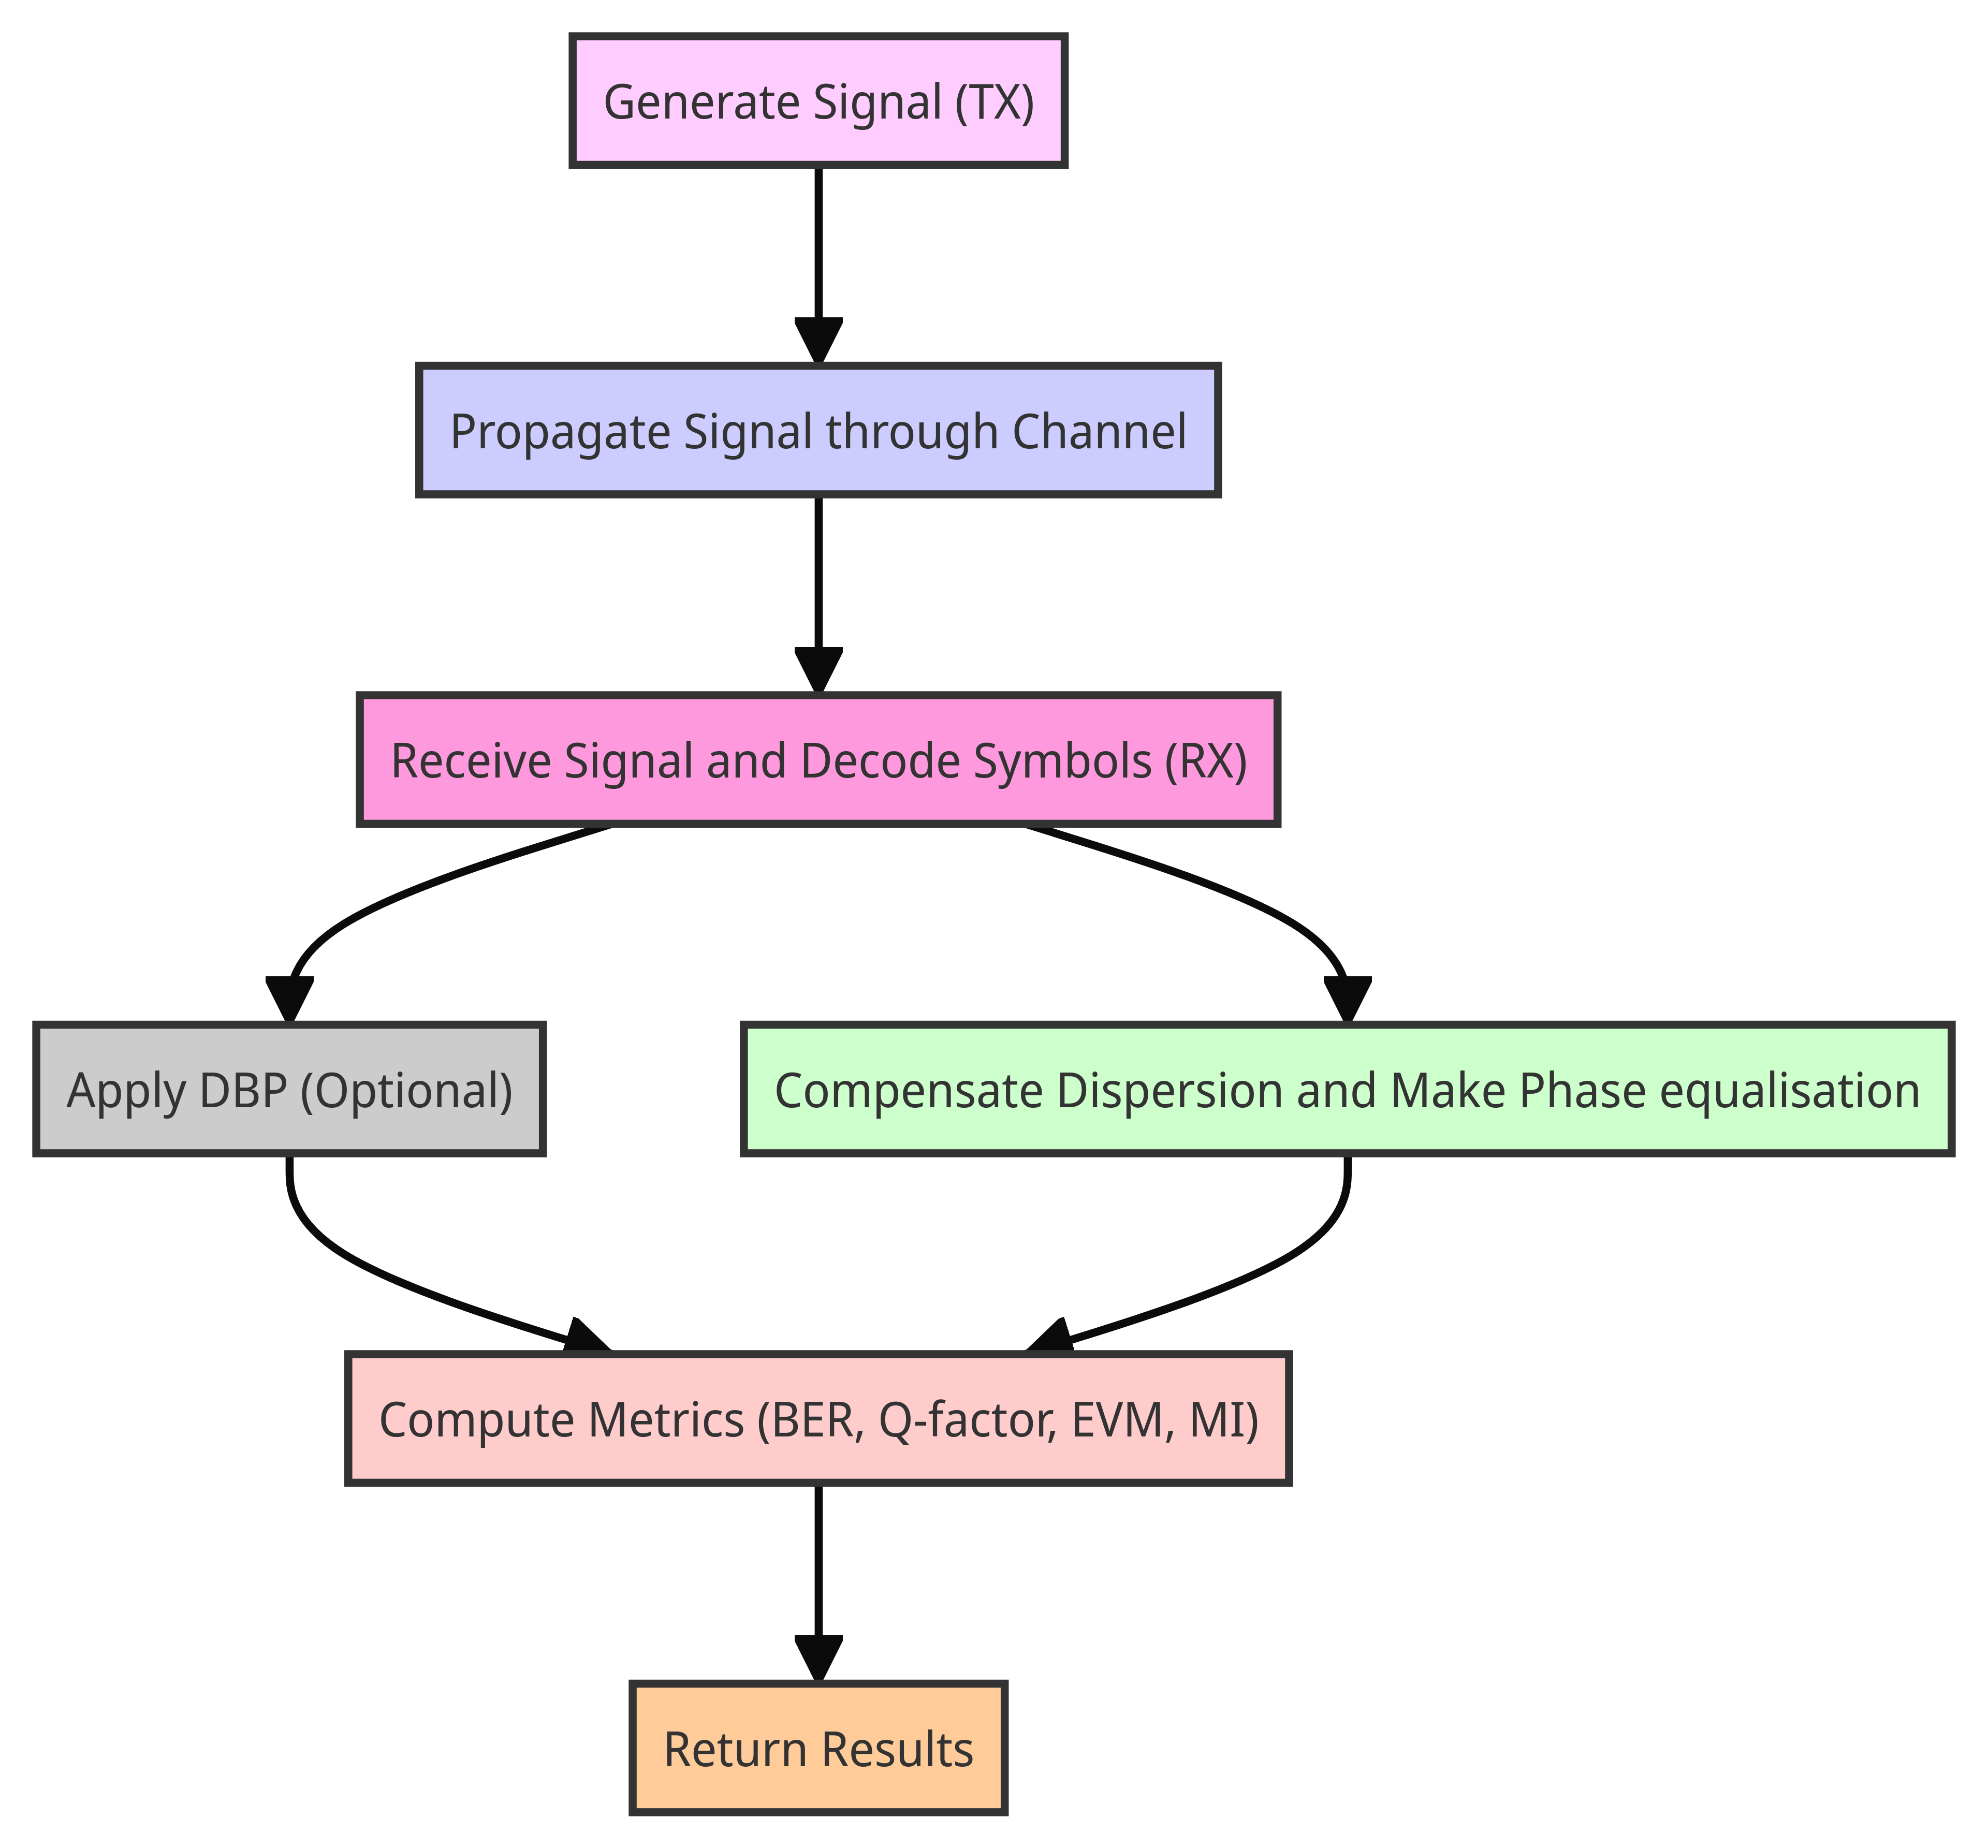
\includegraphics[width=0.7\linewidth]{images/hpcom/hpcom_pipe.png}
    \caption{Framework architecture for optical communication system simulation, featuring optimized transceiver (Tx) design, GPU-accelerated SSFM-based channel model (with $N$ spans of length $L$), receiver implementation (Rx), and performance metrics evaluation including BER, EVM, and MI.}
    \label{fig:hpcom_scheme}
\end{figure}

The proposed framework is built on the TensorFlow 2.x library, with Python as the primary programming language. It is designed to be compatible with the MATLAB environment through the \textrm{pyrun} function, enabling seamless integration with existing MATLAB workflows.

The main components of the framework include the transmitter (Tx), the optical channel model (using \Gls{ssfm} and its higher-order variations), the receiver (Rx), and the metrics evaluation block (see Fig.~\ref{fig:hpcom_scheme}). Besides the aforementioned modules, there are blocks dedicated to compensation and various signal processing techniques. These encompass chromatic dispersion compensation, nonlinear phase equalization, and digital backpropagation. Notably, within these blocks, users have the liberty to incorporate their own \Gls{dsp} techniques or even employ \Gls{ml}-based methods. By default, the transmitter generates a WDM signal with properties as described below. Once the signal is formed by the Tx, it is passed to the second block - the channel model, where a \gls{ssmf} optical channel is simulated with variable numbers of spans and an Erbium-Doped Fiber Amplifier (EDFA) scheme. The Rx consists of a matched filter implementation, chromatic dispersion compensation (CDC), signal demodulation and hard decision blocks. After processing the received information, it can be used to evaluate desired performance metrics such as Bit Error Rate (BER), Error Vector Magnitude (EVM), Mutual Information (MI), or any custom metric.

The Schr\"odinger equation and the Manakov equation (see Eqs.~(\ref{eq:nlse_att}) and~(\ref{eq:manakov_att})) are two widely-used mathematical models that describe light propagation in single-mode optical fibers, taking into account dispersion and nonlinearity effects~\cite{agrawal2000nonlinear}. The Schr\"odinger equation models the evolution of the slowly varying optical field envelope, while the generalized Manakov equation provides a more sophisticated model for light propagation in a two-polarization optical fiber, including polarization-mode dispersion and nonlinear interactions between polarizations~\cite{poletti2008description, mumtaz2012nonlinear}.
HpCom incorporates both of these models, utilizing a GPU-accelerated SSFM implementation for the efficient and accurate simulation of optical communication systems. This forms the core of the framework, ensuring that it can handle complex scenarios and deliver reliable results. Further details on the implementation can be found in the accompanying framework documentation\cite{esf0_2023_7880552}.

By default, our framework employs a classical WDM channel scheme (see Appendix~\ref{sec:hpcom_param} and code examples~\ref{lst:default_channel_param} and~\ref{lst:default_wdm_param}) for SSMF with an EDFA~\cite{essiambre2010capacity}, and ideal transmitter and receiver. However, users can easily customize their channel line by adjusting various parameters for the simulations. For instance, you can explore other types of optical fibers such as TrueWave Classic\cite{taylor2002application} (TWC) or Large Effective Area Fiber\cite{charlet200972} (LEAF) with corresponding parameters. Additionally, you can modify signal parameters to use not only WDM with Quadrature Amplitude Modulation (QAM) but also other types of modulations or signals.


\section{Framework Architecture}

\begin{figure}[t]
   \centering
        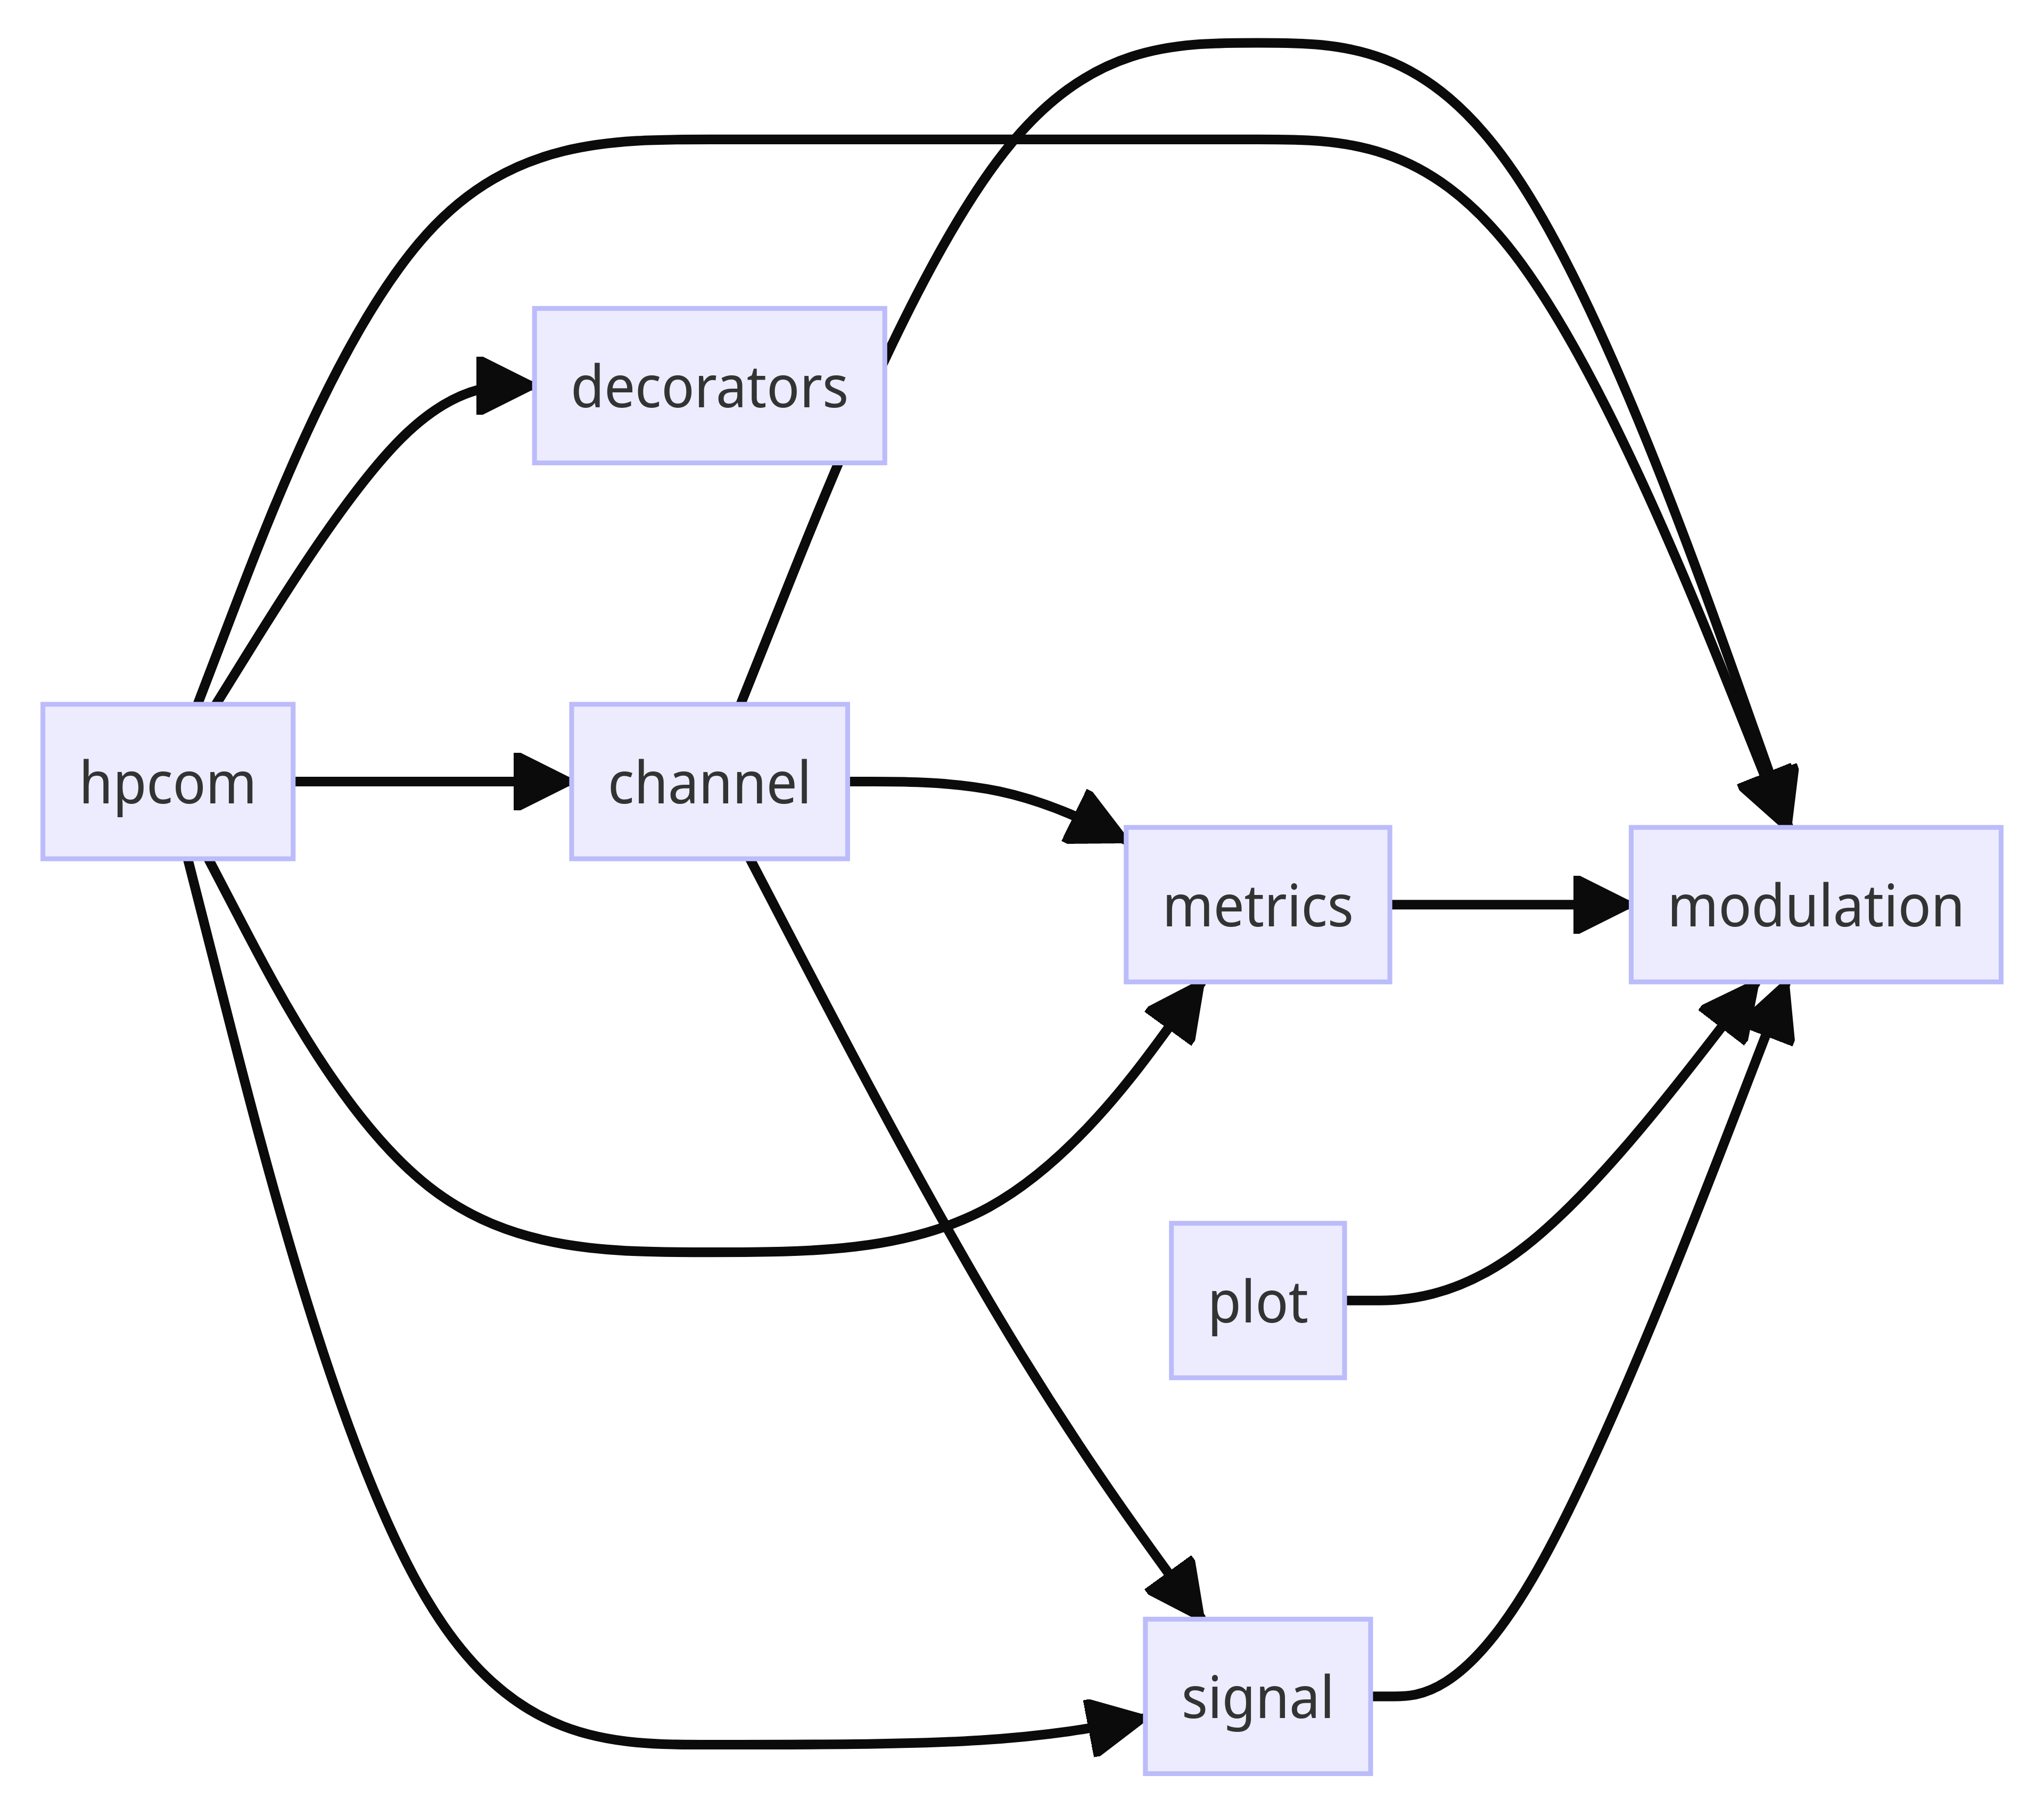
\includegraphics[width=0.7\linewidth]{images/hpcom/hpcom_sctructure.png}
    \caption{Schematic representation of the HpCom library architecture showcasing its modular design for simulating optical communication systems.}
    \label{fig:hpcom_arch}
\end{figure}

\Gls{hpcom} is structured into several integral modules, as illustrated at Fig.~(\ref{fig:hpcom_arch}). Here's a simplified summary of the modules and their functionalities:

\begin{description}[style=multiline, leftmargin=2.5cm, font=\normalfont]
    \item[\texttt{channel}] This module facilitates the establishment of channel parameters such as the length of each span, dispersion, nonlinearity, etc., and provides GPU-accelerated simulation of the optical channel.
    \item[\texttt{signal}] Engaged in the generation and decoding of Wavelength Division Multiplexing (WDM) or Orthogonal Frequency Division Multiplexing (OFDM) signals.
    \item[\texttt{modulation}] This module is responsible for data modulation, creation of constellations, and modulation/demodulation with various Quadrature Amplitude Modulation (QAM) formats (16-, 64-, 256-, 1024-QAM).
    \item[\texttt{metrics}] Metrics module houses optimized functions necessary for computing performance metrics such as Bit Error Rate (BER), Mutual Information (MI), Error Vector Magnitude (EVM), Q-factor or any user-defined metrics. These metrics are essential for evaluating the performance of the communication system.
    \item[\texttt{plot}] This supplementary module aids in technical plotting, providing a visual representation of data and system performance.
    \item[\texttt{decorators}] An additional utility module. It provides python decorators which can enhance the functionality or performance of the code.
\end{description}

\subsection{Channel Module}
The \texttt{channel} module in the \texttt{hpcom} framework is pivotal for the simulation of signal propagation through a fiber optic channel. It primarily relies on the nonlinear Schrödinger equation (NLSE) or the Manakov equation to model the propagation dynamics. This module encompasses two main functions: \texttt{full\_line\_model\_wdm} and \texttt{full\_line\_model\_ofdm}, which are designed for Wave Division Multiplexing (WDM) and Orthogonal Frequency Division Multiplexing (OFDM) signal generation and propagation, respectively.

This module contains several other functions, as enumerated below:
\begin{description}[style=multiline, leftmargin=7.7cm, font=\normalfont]
    \item[\texttt{get\_default\_channel\_parameters}] Constructs a dictionary populated with default channel parameters.
    \item[\texttt{update\_channel\_parameters}] Modifies the channel parameters and recalculates internal characteristics to mitigate errors, especially in scenarios where the user overlooks the necessity of manual recalculation.
    \item[\texttt{update\_channel\_parameters\_from\_json}] Initializes default channel parameters, then loads and updates any existing parameters from a specified JSON file.
    \item[\texttt{create\_channel\_parameters}] Generates a dictionary with user-provided channel parameters and computes additional values requisite for simulations.
\end{description}
For a comprehensive overview, refer to Appendix~\ref{sec:hpcom_param}. The functions \texttt{transceiver\_line\_model} and \texttt{receiver\_model} are further discussed in the following subsection.


\subsubsection{Functions \texttt{full\_line\_model\_wdm} and \texttt{full\_line\_model\_ofdm}}
The function \texttt{full\_line\_model\_wdm} serves as a comprehensive model encompassing signal generation, propagation, reception, demodulation, and metrics computation. Below is a description of the primary parameters:

\begin{description}[style=multiline, leftmargin=4.5cm, font=\normalfont]
    \item[\texttt{channel}] A dictionary containing the channel model parameters (see Appendix~\ref{sec:hpcom_param} for more details).
    \item[\texttt{wdm}] A dictionary containing the parameters of the WDM signal (see Appendix~\ref{sec:hpcom_param} for more details).
    \item[\texttt{bits} (optional)] Utilized when a specific bit sequence is to be transmitted.
    \item[\texttt{points} (optional)] Utilized when predefined points are available\footnote{The \texttt{points} must be scaled in accordance with the average signal power, refer to the scaling subsection.}.
    \item[\texttt{channels\_type} (default: 'all')] Specifies whether metrics should be computed for all WDM channels or only the middle channel.
    \item[\texttt{verbose} (default: 0)] Controls the verbosity level of messages, with 0 being minimal verbosity and higher values displaying more information\footnote{The current maximum verbosity level is 3, subject to change in future versions.}.
    \item[\texttt{dbp} (default: False)] A flag to toggle \gls{dbp} calculations.
    \item[\texttt{dbp\_parameters} (optional)] Defines the parameters for \Gls{dbp} (see Appendix~\ref{sec:hpcom_param} for more details).
    \item[\texttt{optimise} (default: 'not')] When set to a parameter ('ber\_x', 'evm\_x', 'mi\_x'), the function returns only the value for this parameter. Otherwise, function returns all available information (see information below).
    \item[\texttt{ft\_filter\_values\_tx} (optional)] The Fourier coefficients corresponding to filter values for the transmitter are specified through this parameter. In scenarios where a non-standard filter shape is employed (i.e., a shape divergent from the Root Raised Cosine (RRC) filter), users have the liberty to define the Fourier modes of the filter explicitly.
    \item[\texttt{ft\_filter\_values\_rx} (optional)] Fourier coefficients of filter values for the receiver. Same functionality as for \texttt{ft\_filter\_values\_tx}.
\end{description}

The function \texttt{full\_line\_model\_ofdm} adheres to a similar logic as \texttt{full\_line\_model\_wdm}, with a few distinctions. Specifically, it accepts an \texttt{ofdm} dictionary to cater to the parameters requisite for \Gls{ofdm} signal processing. Unlike \texttt{full\_line\_model\_wdm}, this function does not use the \texttt{channels\_type}, \texttt{ft\_filter\_values\_tx}, and \texttt{ft\_filter\_values\_rx} parameters.


Both functions can operate in either single or dual polarization mode. In a single polarization scenario, only the x-polarization is used, while in dual polarization, both x and y polarizations are employed. The functions returns various metrics such as Bit Error Rate (BER), Q-factor, Error Vector Magnitude (EVM), and Mutual Information (MI), alongside the constellation points at various stages of the transmission link.

The \texttt{full\_line\_model\_wdm} and \texttt{full\_line\_model\_ofdm} functions return a dictionary of results when the \texttt{optimise} parameter is set to 'not'. The keys in this dictionary, along with their descriptions, are provided below:

\begin{description}[style=multiline, leftmargin=4cm, font=\normalfont]
    \item[\texttt{points\_orig}] The original points at the transmitter.
    \item[\texttt{points\_noneq}] The constellation points at the receiver, post the matched Root Raised Cosine (RRC) filtering for \acrshort{wdm} and post \acrshort{fft} for \acrshort{ofdm}, but prior to any equalization.
    \item[\texttt{points}] The constellation points after chromatic dispersion compensation.
    \item[\texttt{points\_shifted}] The constellation points after chromatic dispersion compensation and nonlinear phase equalization.
    \item[\texttt{points\_found}] The constellation points found after hard-decision.
    \item[\texttt{ber}] The Bit Error Rate (BER) for transmitted points.
    \item[\texttt{q}] The Q-factor for transmitted points.
    \item[\texttt{evm}] The Error Vector Magnitude (EVM) for transmitted points.
    \item[\texttt{mi}] The Mutual Information (MI) for transmitted points.
\end{description}

If the \texttt{dbp} flag is set to True, indicating that digital backpropagation is to be computed, additional keys are included in the result dictionary:

\begin{description}[style=multiline, leftmargin=4cm, font=\normalfont]
    \item[\texttt{points\_dbp}] The constellation points post digital backpropagation.
    \item[\texttt{ber\_dbp}] The BER post digital backpropagation.
    \item[\texttt{q\_dbp}] The Q-factor post digital backpropagation.
    \item[\texttt{evm\_dbp}] The EVM post digital backpropagation.
    \item[\texttt{mi\_dbp}] The MI post digital backpropagation.
\end{description}

This organized return structure allows for a thorough analysis of the constellation at the receiver at various stages of post-processing, and facilitates the evaluation of the \Gls{dbp}'s impact on the signal transmission quality metrics.


\subsubsection{Functions \texttt{transceiver\_line\_model} and \texttt{receiver\_model}}
To accommodate a more flexible tuning of the channel model, two distinct functions are provided: \texttt{transceiver\_line\_model} and \texttt{receiver\_model}. The former is devoted to the generation of the WDM signal and its propagation through the link, without receiver component, while the latter serves as a receiver for the WDM signal outputted from the fiber model.

The function \texttt{transceiver\_line\_model} facilitates the creation and transmission of a WDM signal through the link, albeit without engaging the receiver functionality. For a comprehensive understanding of the function's inputs, refer to the description provided in the preceding subsection concerning the \texttt{full\_line\_model\_wdm} function.

\begin{lstlisting}[language=Python, caption=Usage of \texttt{transceiver\_line\_model} function, label=lst:tx_line_model]
result = transceiver_line_model(channel, wdm, bits=None, points=None, verbose=0, dbp=False, ft_filter_values_tx=None)
# result contains:
# result = {
#  'signal': [signal_x, signal_y],  # x- and y-polarisations after propagation
#  'points_orig': [points_x_orig, points_y_orig],  # transmitted points for x- and y-
#  'ft_filter_values': [ft_filter_values_x, ft_filter_values_y]  # Fourier coefficients for filter used to create WDM signal for x- and y-
#         }
\end{lstlisting}

The function \texttt{receiver\_model} operates as the receiver, taking the WDM signal from the fiber model's output. It employs a matched Root Raised Cosine (RRC) filter to extract the constellation points, subsequently performing Chromatic Dispersion Compensation (CDC) and Nonlinear Phase Equalization (NPE), followed by metrics computation. Similar to transceiver model, the input parameters for this function have the same meaning as for \texttt{full\_line\_model\_wdm}, as detailed in the previous subsection.

\begin{lstlisting}[language=Python, caption=Usage of \texttt{receiver\_model} function, label=lst:rx_model]
result = receiver_model(wdm, signal, points_orig, ft_filter_values_rx, channels_type='all', verbose=0, optimise='not')
# result same as for full_line_model_wdm function
\end{lstlisting}

In the current version of the HpCom package, support is extended exclusively to WDM. However, forthcoming iterations will encompass support for OFDM, thereby broadening the scope and applicability of these functions.


\subsection{Signal Module}
The Signal Module encompasses key functionalities pertinent to both Wavelength Division Multiplexing (WDM) and Orthogonal Frequency Division Multiplexing (OFDM) signal generation and decoding. For an introductory exposition on WDM and OFDM, the reader is directed to Section~\ref{sec:signals}.


\subsubsection{WDM Signal Generation and Demodulation}

\begin{figure}[t]
   \centering
        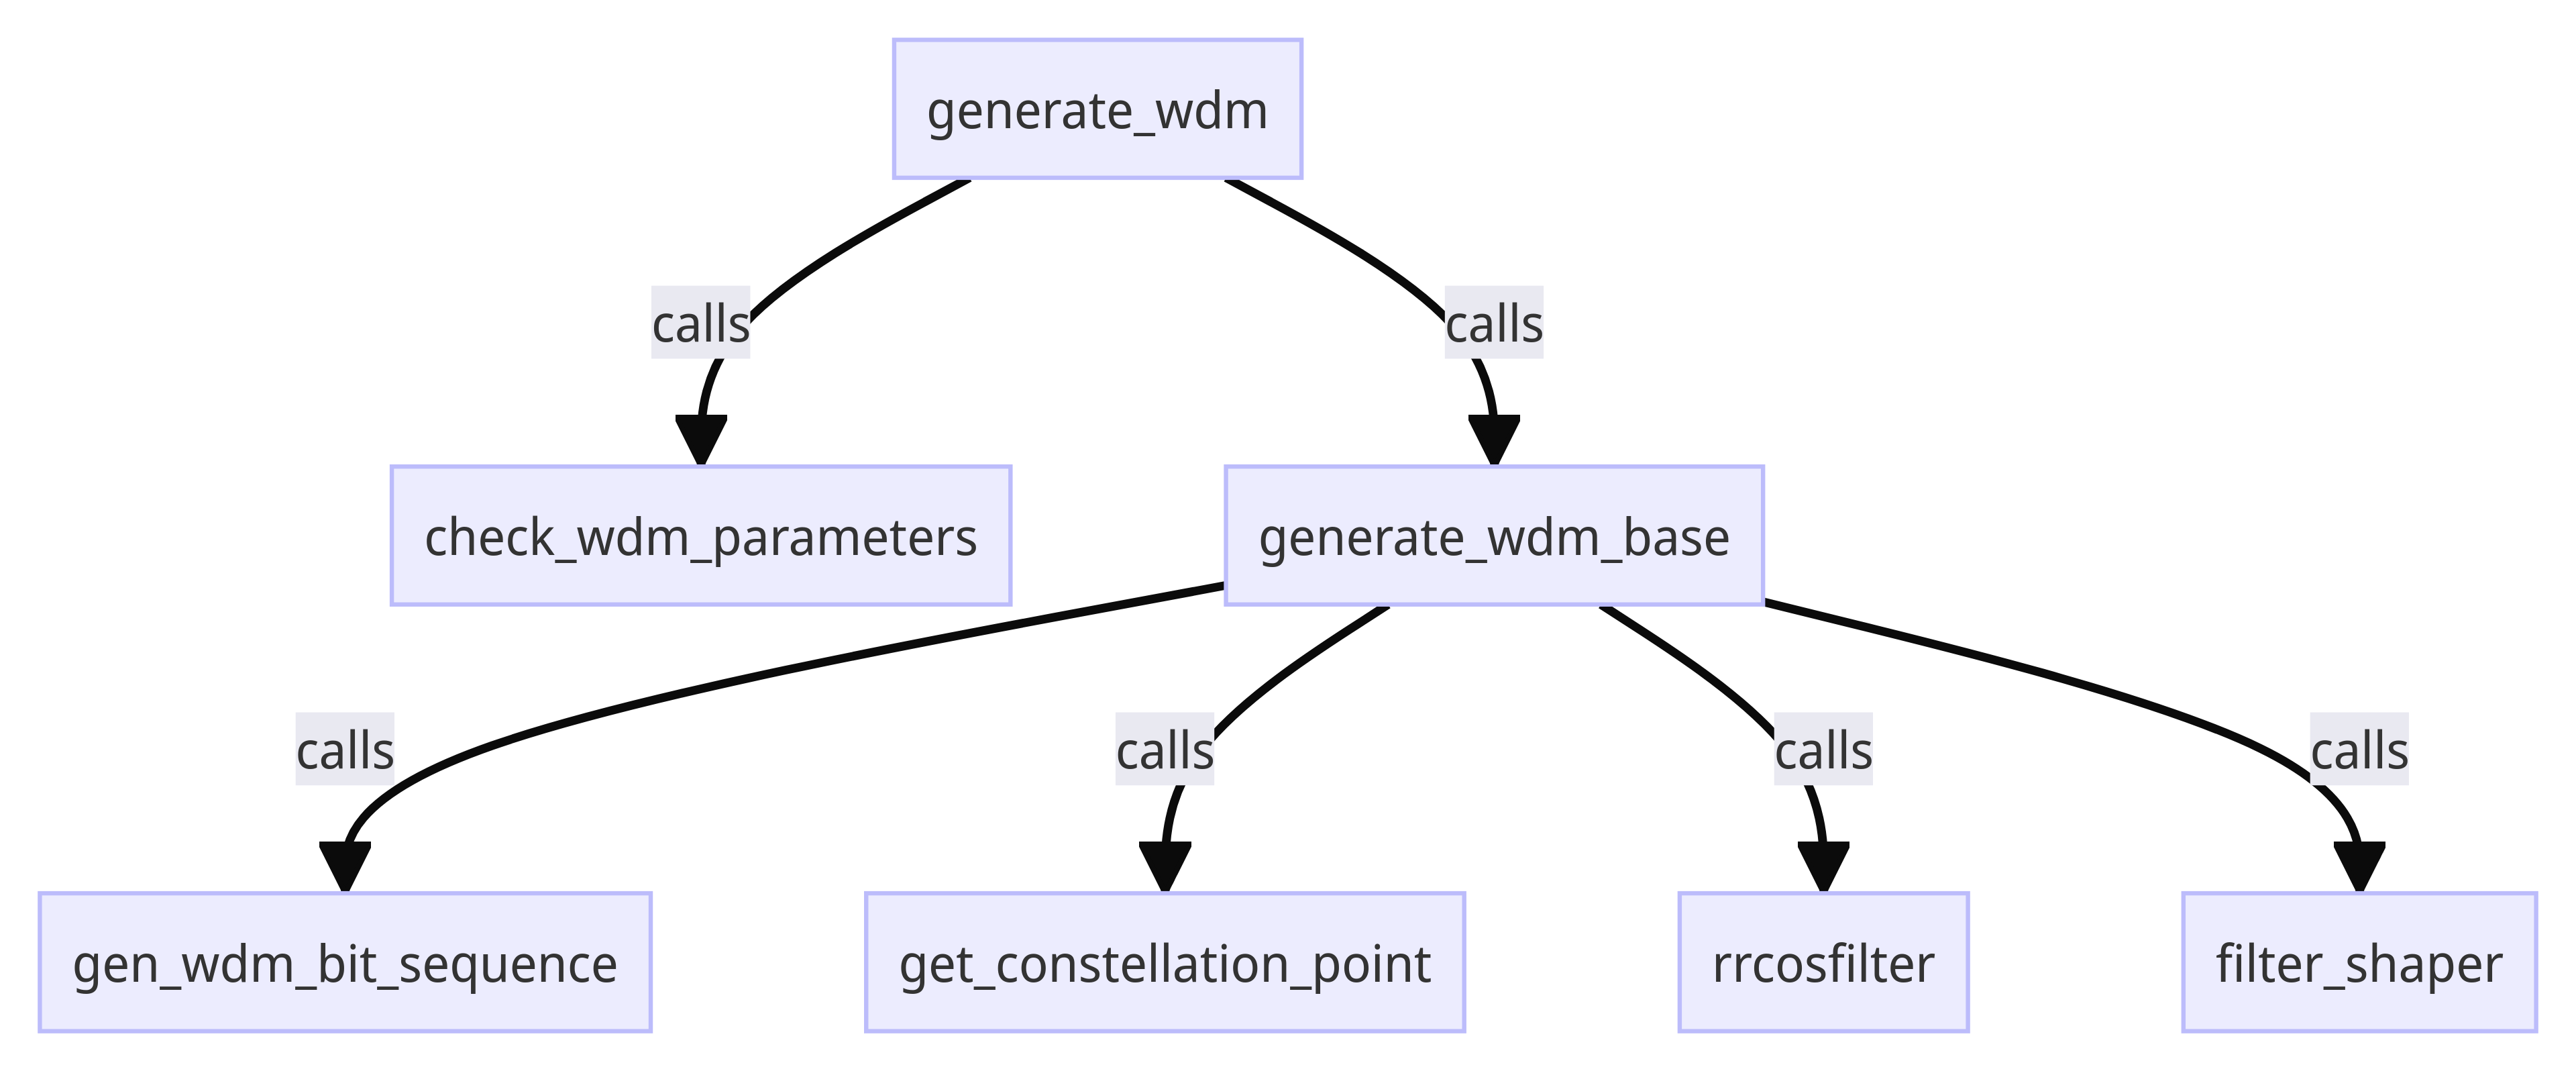
\includegraphics[width=0.8\linewidth]{images/hpcom/wdm_generation.png}
    \caption{Scheme of WDM generation.}
    \label{fig:wdm_generation}
\end{figure}

The principal function for WDM signal generation is given by:
\begin{lstlisting}
signal, info = generate_wdm(wdm, bits=None, points=None, ft_filter_values=None)
\end{lstlisting}
This function orchestrates the signal generation process. Initially, it checks if the \texttt{bits} or \texttt{points} parameters are provided; if absent, it generates them based on the stipulated parameters in the \texttt{wdm} dictionary, such as average signal power or modulation format. The \texttt{points} are scaled in accordance with the average signal power (details in the Appendix~\ref{sec:scaling}).

Subsequently, for each wavelength, the function invokes a subroutine \texttt{generate\_wdm\_base},
which manages the generation process for a single wavelength within the current bandwidth. The modulated points (e.g., 16-QAM) are taken, and zeros are interspersed between them according to the specified upsampling rate. For instance, with an upsampling rate of 1, every sample corresponds to a constellation point; with a rate of 2, every other sample is a constellation point, with zeros in between, etc.

The convolution operation, as delineated in Eq.~\ref{eq:wdm_nlse}, is central to this process. Leveraging the Fourier Transform, the convolution is transmuted into a multiplication operation in the frequency domain, which is amenable to GPU acceleration. The Fourier spectra of the upsampled points array and the filter are multiplied. Although a \Gls{rrc} filter is typically utilized, the implementation accommodates user-defined filter shapes.

This procedure is reiterated for each WDM channel, engendering the complete WDM signal with a distinct frequency shift for the Fourier spectrum of each channel, as dictated by the \texttt{wdm['channel\_spacing']} parameter. The convolution operation is executed via the following functions, catering to both time and frequency domain signals:
\begin{lstlisting}
def filter_shaper_spectral(spectrum, ft_filter_val):
 return tf.signal.ifftshift(tf.signal.ifft(tf.signal.ifftshift(spectrum * ft_filter_val)))

def filter_shaper(signal, ft_filter_val):
 spectrum = tf.signal.fftshift(tf.signal.fft(signal))
 return filter_shaper_spectral(spectrum, ft_filter_val)
\end{lstlisting}

With the WDM signal now generated, decoding the constellation necessitates retracing the aforementioned steps in reverse order. As delineated in Section~\ref{sec:signals}, the application of a matched filter, as illustrated in Eq.~(\ref{eq:wdm_matched_filter}), is imperative for this process. In the code, this operation is executed by the function \texttt{receiver\_wdm}, which in turn invokes \texttt{matched\_filter\_wdm}. The latter essentially performs the following actions: it isolates each WDM channel in the frequency domain (the channel separation is dictated by the \texttt{wdm['channel\_spacing']} parameter), and applies the matched filter to the resultant signal (or spectrum, as reverting to the time domain is not feasible, thus the truncated spectrum is utilized). This matched filtering operation employs the previously referenced \texttt{filter\_shaper\_spectral} function. The ultimate output of this process are the decoded constellation points. Note that these points are identified prior to the hard decision stage, hence, they can be dispersed across the complex constellation plane.



\subsubsection{OFDM Signal Generation and Demodulation}

\begin{figure}[thpb]
   \centering
    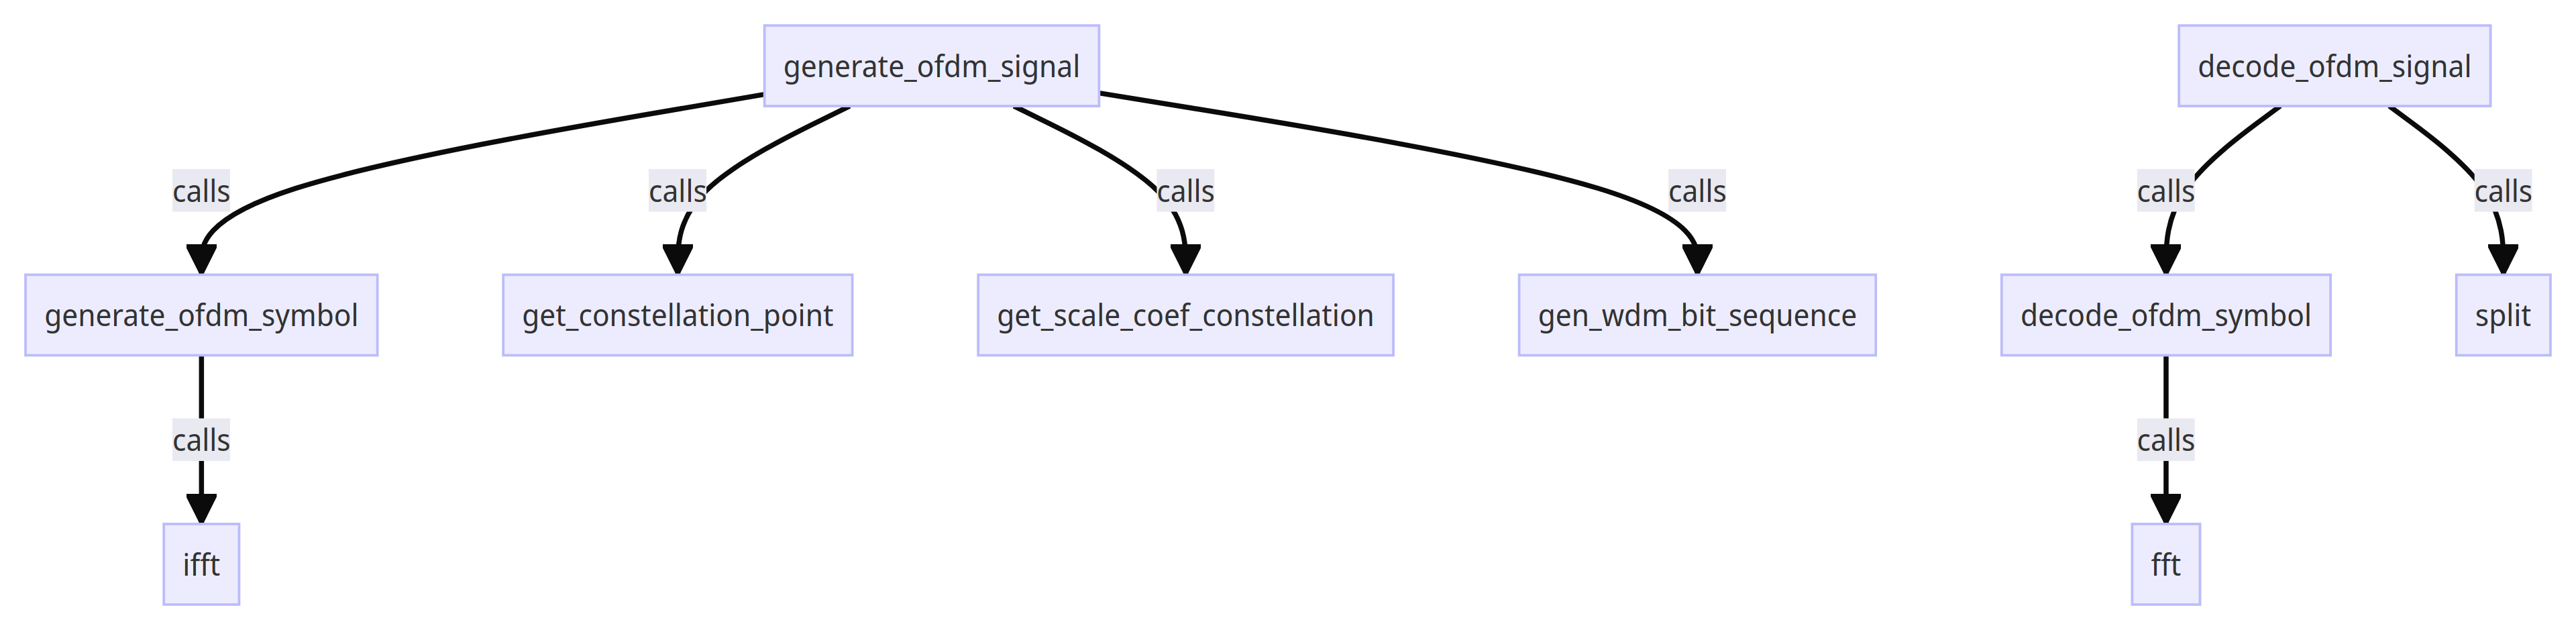
\includegraphics[width=1\linewidth]{images/hpcom/odfm_creation.png}
    \caption{Scheme of OFDM signals generating and decoding.}
    \label{fig:ofdm_code_scheme}
\end{figure}

The generation of an OFDM symbol is undertaken by the function \texttt{generate\_ofdm\_symbol}, where, based on the provided or generated bits, constellation points are derived. These points are then subjected to an Inverse Fast Fourier Transform (IFFT) operation to transition from the frequency domain to the time domain, thereby forming the OFDM symbol. If specified, a cyclic prefix is appended to this symbol to mitigate inter-symbol interference. 

Subsequently, the \texttt{generate\_ofdm\_signal} function orchestrates the overall generation of the OFDM signal. It initiates by configuring the average power of the signal, especially in scenarios involving two polarizations. A loop iterates through each polarization, within which the bits are either provided or generated anew, followed by the derivation of constellation points. The \texttt{generate\_ofdm\_symbol} function is invoked within this loop to generate the requisite OFDM symbols which are then concatenated to form the complete OFDM signal for the corresponding polarization. This function mirrors the procedural blueprint of OFDM signal generation, extending from bit generation to the aggregation of OFDM symbols.

\begin{lstlisting}
signal, info = generate_ofdm_signal(ofdm_init, bits_init=None, points_init=None, seed=0)
\end{lstlisting}

On the receiving end, the \texttt{decode\_ofdm\_symbol} function is engaged to demodulate a single OFDM symbol. It begins by discarding the cyclic prefix, if present, and then conducts a Fast Fourier Transform (FFT) operation on the OFDM symbol to revert back to the frequency domain, extracting the constellation points.

The broader demodulation of the entire OFDM signal is managed by the \texttt{decode\_ofdm\_signal} function. It dissects the received OFDM signal into individual OFDM symbols, and invokes \texttt{decode\_ofdm\_symbol} for each symbol to retrieve the constellation points. The collected points from all symbols and polarizations are then returned as the output, marking the completion of the OFDM signal demodulation process.

\begin{lstlisting}
points = decode_ofdm_signal(ofdm_signal, ofdm)
\end{lstlisting}


% \subsection{Metrics and Modulation}

% Do we need it??


\section{Performance Evaluation}

\begin{figure*}[t]
   \centering
    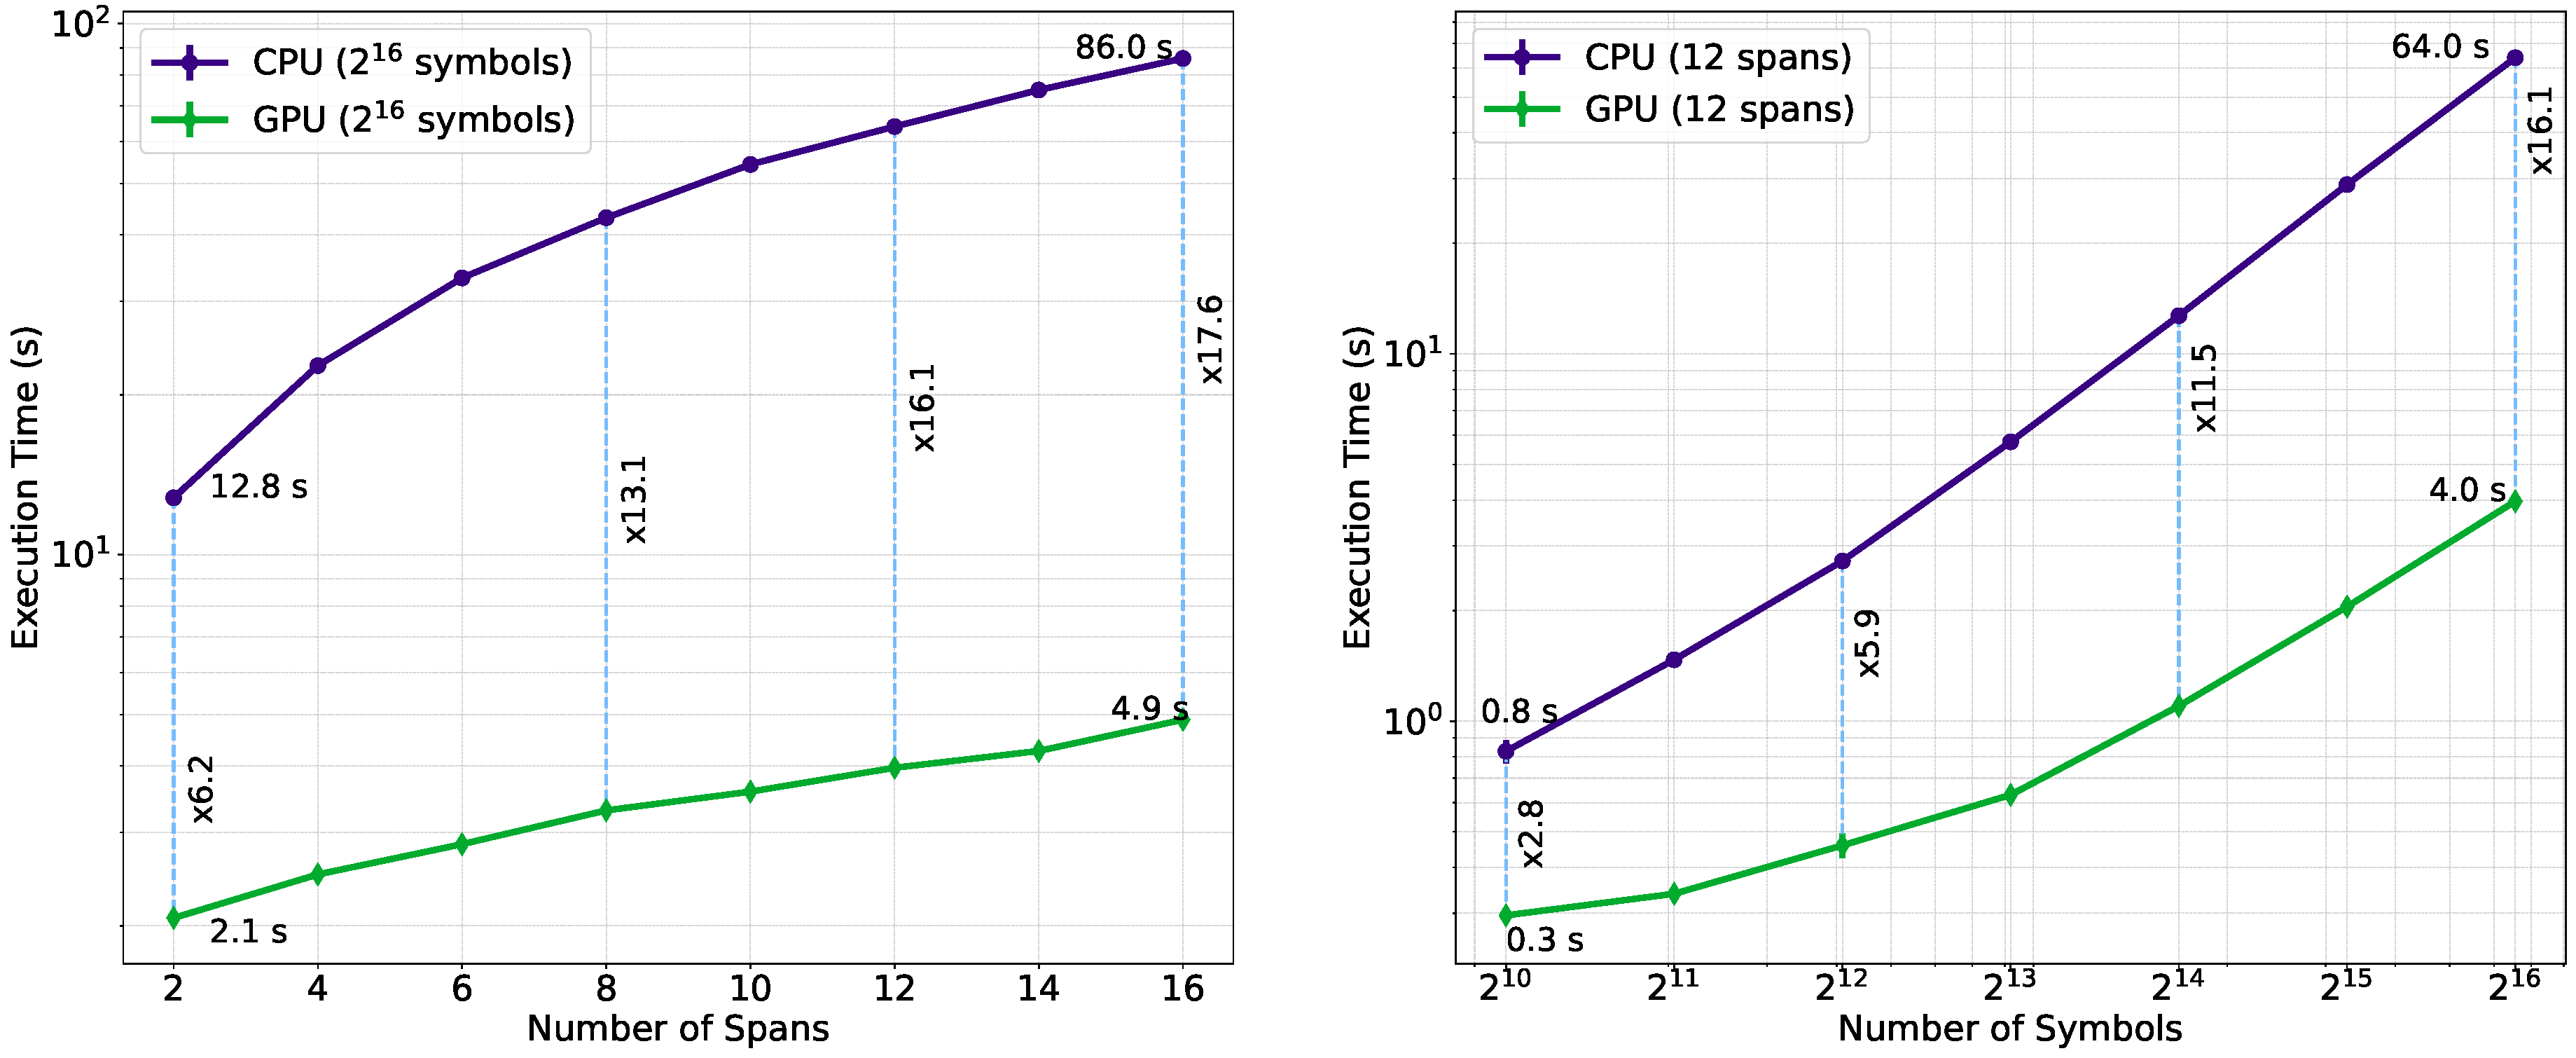
\includegraphics[width=1\linewidth]{images/hpcom/total.pdf}
    \caption{The left figure displays the total execution time for all steps of the optical channel simulation with $2^{16}$ symbols, comparing single CPU core and GPU usage, as a function of the number of spans (SMF, each span is 80 km). The right figure illustrates the relationship between execution time for a single CPU core and GPU usage with a fixed number of spans and varying number of symbols in the simulation.}
    \label{fig:total}
\end{figure*}

To evaluate the framework's performance, we conducted several tests comparing computation time between CPU and GPU. The signal used was a two-polarization 64-QAM WDM with 1 km per step and 80 km span. The SSMF fiber parameters were: $\gamma$ = 1.2 (W$\cdot$ km)$^{-1}$, $D$ = 16.8 ps/(nm$\cdot$km), and $\alpha$ = 0.21 dB/km. At the end of each span, optical fiber losses were compensated using an EDFA with a 4.5 dB noise figure. The benchmark calculations were performed using an NVIDIA GeForce RTX 3070 with 8GB GDDR6 and a single core of an AMD Ryzen 9 5900HX with up to 4.6GHz.

The total simulation time consists of four components: the transmitter (Tx) simulation time $T_{Tx}$, channel simulation time $T_{channel}$, receiver (Rx) simulation time $T_{Rx}$, and metrics evaluation time $T_{metrics}$. In the current implementation, Tx, Rx, and metrics calculations utilize CPU cores, but employ optimized functions to prevent $O(n^2)$ computational complexity. For instance, with $2^{15}$ symbols, Tx, Rx, and metrics calculations take approximately 200 ms, significantly less than the propagation time (1230 ms for GPU and 27000 ms for CPU). Optimal results are observed when working within the available GPU memory. When the number of simulation points equals $\mathrm{n\_symbols} \cdot \mathrm{upsampling} = 2^{16} \cdot 2^{4}$, the overall memory required for calculations is around 6.5 GB. To perform more precise simulations for multi-channel WDM signals, one must control the overall number of points or employ more advanced hardware.

Figure~\ref{fig:total} displays the dependence of total execution time on the number of spans for a fixed number of symbols (left), and the dependence of total execution time on the number of symbols with fixed propagation length (right). The graphs indicate that as the number of spans or symbols increases, the GPU's speedup factor also grows. For instance, for $2^{16}$ symbols and 16 spans, the GPU is 17 times faster.

We also evaluated the system performance for an extreme case, where the total memory required significantly exceeds the GPU's capacity. We conducted simulations with $2^{19}$ symbols (eight times more memory than the current GPU) and separately assessed the time for each component of the simulations (Fig.~\ref{fig:propagation_time}). The graph demonstrates that the gain is independent of the propagation length, as expected, and remains approximately 34 times faster on the GPU compared to the CPU. However, for long propagation lengths (or more steps per span), the total time saved is substantial, as the GPU completes the simulation in under a minute (53.8 s), while the CPU takes over 30 minutes.

\begin{figure}[t]
   \centering
        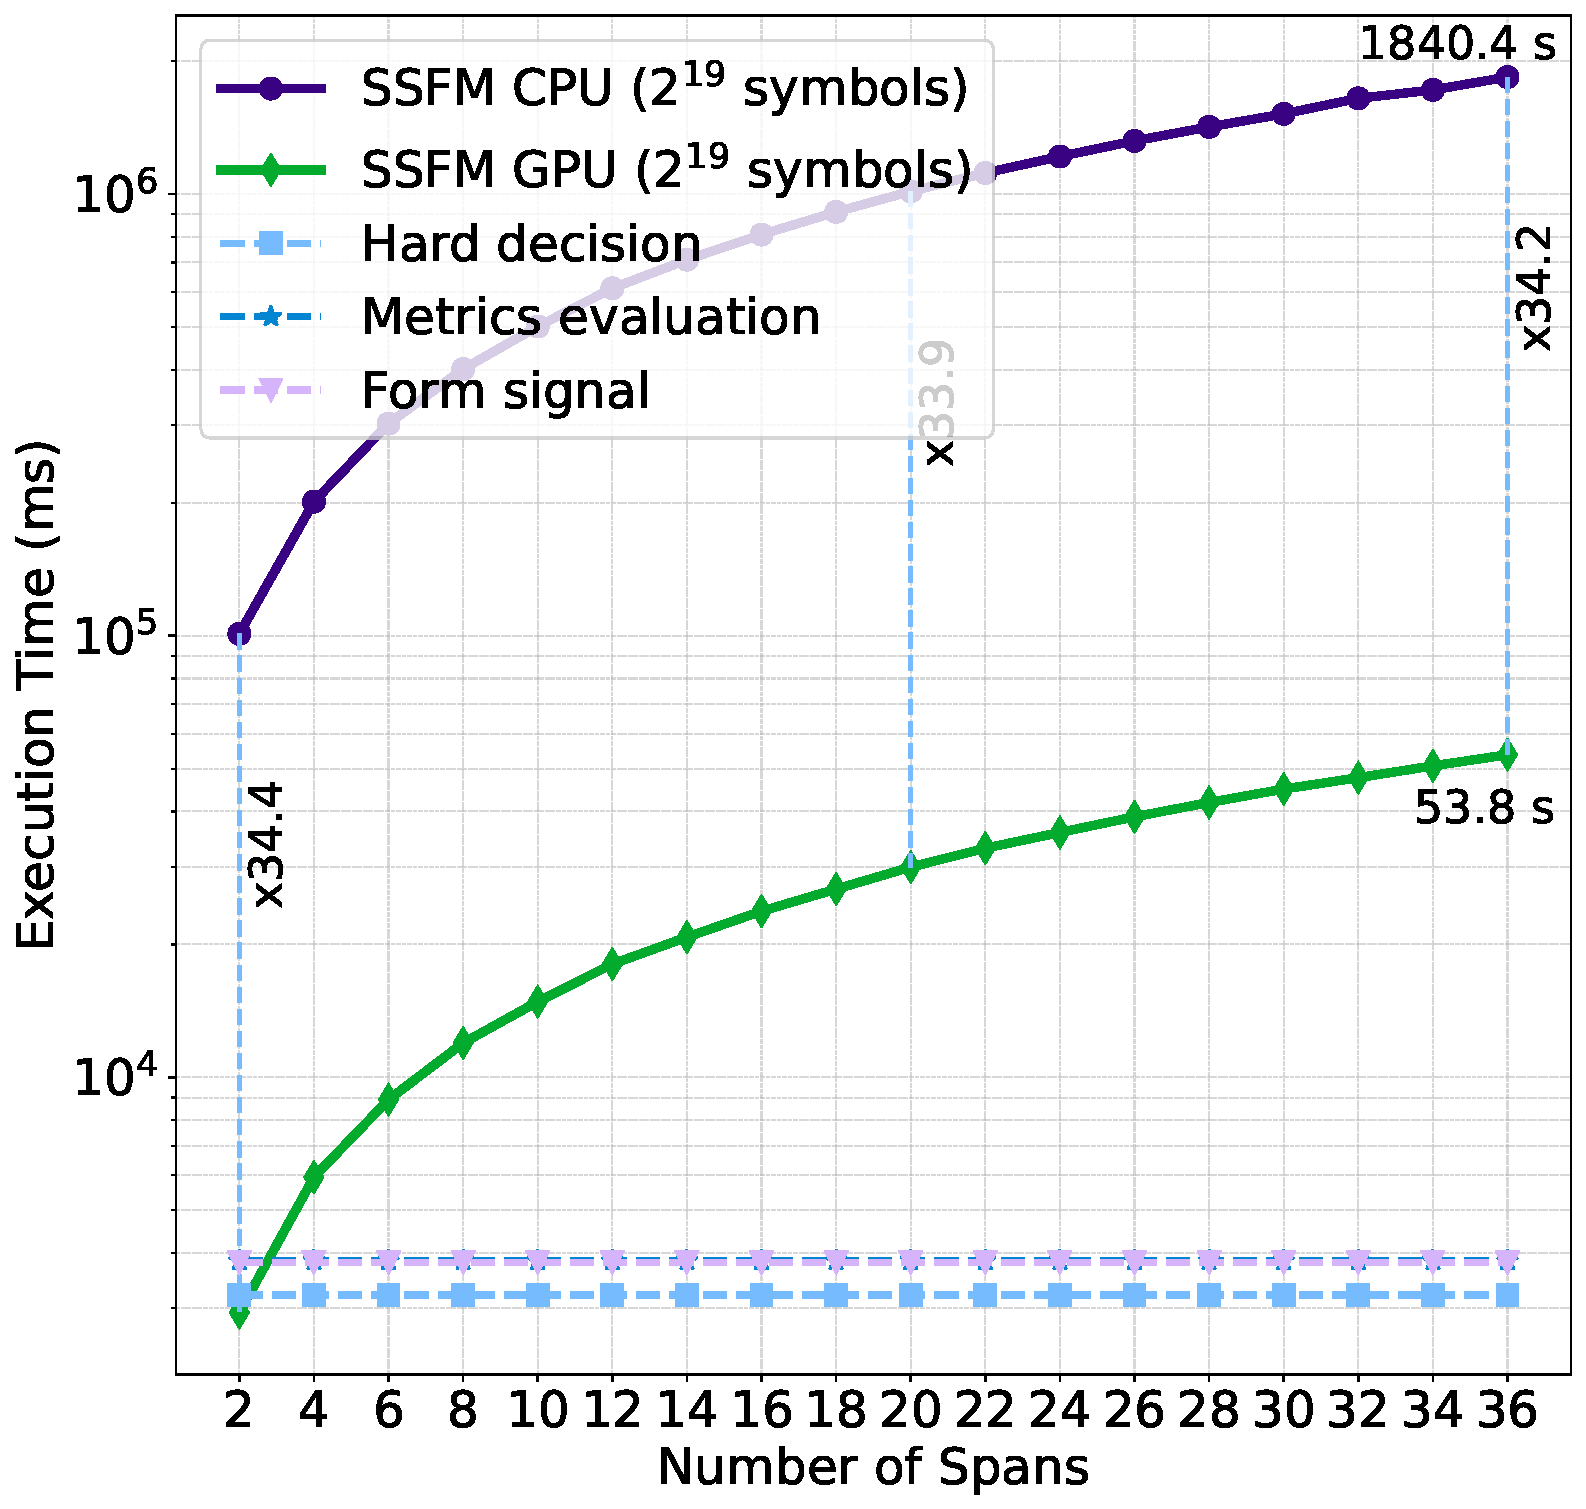
\includegraphics[width=0.6\linewidth]{images/hpcom/propagation.pdf}
    \caption{Execution time in milliseconds for various simulation steps as a function of the number of spans. Signal formation at the Tx, hard decision at the Rx, and metric evaluation (e.g., BER, EVM, MI) rely on the CPU and are influenced by the number of symbols, depicted as dashed lines. Propagation, which is performed on either the CPU or GPU, is represented by solid lines.}
    \label{fig:propagation_time}
\end{figure}

% The results were obtained by measuring the execution time of both implementations for various problem sizes (n\_symbols) while keeping the number of fiber spans (n\_spans) constant at 12. The mean execution time and standard deviation were calculated over multiple runs (7 runs for most cases) to ensure the accuracy of the results.

% Upon analyzing the graph, we observe that the GPU execution times are consistently lower than the CPU execution times across all problem sizes. Furthermore, the difference in execution times between the two implementations increases as the problem size grows, indicating that the GPU-accelerated framework becomes more advantageous for larger problems.

% Specifically, the speedup achieved by the GPU implementation relative to the CPU implementation ranges from approximately 2.8x for smaller problem sizes (n\_symbols = 2 ** 10) to around 16.1x for larger problem sizes (n\_symbols = 2 ** 16). This trend suggests that the GPU-accelerated framework is particularly well-suited for large-scale simulations or scenarios where rapid computation is required.

% In conclusion, the graph clearly demonstrates the superior performance of the GPU-accelerated framework compared to the CPU-based implementation, particularly for larger problem sizes. The increased speedup achieved with the GPU implementation highlights the benefits of utilizing GPU acceleration for optical communication system simulations.


\section{Example of Data Mining}

% Signal propagation in a setup characterized by: model for \gls{smf}, each span is 80 km, \acrshort{wdm} (some cases have single channel and single polarisation, some has multiple channels) with RRC roll-off equal to 0.1. Symbol frequency is 34 GBd, channel spacing is 75GHz. The average signal power $P_{ave}$ varies from  at $-15$ up to $15$ $\textrm{dBm}$, utilizing a 16 or 256-\gls{qam} format. An attenuation coefficient $\alpha = 0.2$ $[\textrm{dB}/\textrm{km}]$, an EDFA noise figure of 4.5 $[\textrm{dB}]$ (some cases has no additional noise from EDFA), a dispersion coefficient $D = 16.8$ $\textrm{ps}/[\textrm{nm} \cdot \textrm{km}]$, and a nonlinear coefficient $\gamma = 1.2$ $[\textrm{W} \cdot \textrm{km}]^{-1}$. 

Our research examines signal transmission in an optical system that includes a model for \gls{smf} with each section being 80 km long. We use \acrshort{wdm}, which in this scenarios involves a single channel and single polarization. The system employs a root-raised cosine (RRC) filter with a roll-off factor of 0.1. We transmit signals at a rate of 34 Gbaud (GBd), with channels spaced 75 GHz apart. The setup has an attenuation coefficient \( \alpha = 0.2 \) dB/km, an EDFA noise figure of 4.5 dB (though some cases do not include additional EDFA noise), a dispersion coefficient \( D = 16.8 \) $\textrm{ps}/[\textrm{nm} \cdot \textrm{km}]$, and a nonlinear coefficient $\gamma = 1.2$ $[\textrm{W} \cdot \textrm{km}]^{-1}$. 


% Figure~\ref{fig:hpcom_example1} and ~\ref{fig:hpcom_example2} show an example of data generation using HpCom, more specifically the illustrate an example of \acrshort{ber} calculation for range of parameters. Lenght of the fiber changes from 80 km to 2000 km (from 1 span of fibre up to 25 spans). Signal average power changes from -15 dBm up to 15 dBm (with step of 0.5 dBm). Left column represents the case where there is no additional EDFA noise, right column - 4.5 dB EDFA noise figure. For each set of parameters there is $2^{16}$ symbols. Figure~\ref{fig:hpcom_example1} shows the case for 16-\acrshort{qam} while Fig.~\ref{fig:hpcom_example2} shows a \acrshort{wdm} signal with 256-\acrshort{qam}. In both pictures first and second rows illustrates dependace of \acrshort{ber} of distance and average power, while first row shows 3d visualisation, second row shows it's 2d projection (colormap). Third row repeats the second raw but with other scale: white regions are correspond to the case when \acrshort{ber} below $10^{-6}$ or above $10^{-1}$. For both Figs. left column represents the case without additional noise from \gls{edfa} and rigth column shows 4.5 dB EDFA noise figure. For left column, as it has to be, when signal power is low, nonlinear effects are neglectible and we have better \acrshort{ber} than in case of noise presence when for small signal power noise significantly corrupts the signal, so then also quality.

Figures~\ref{fig:hpcom_example1} and ~\ref{fig:hpcom_example2} provide examples of data generated with HpCom, highlighting how the \acrshort{ber} is calculated for a range of parameters. The fiber length varies from 80 km to 2000 km, equivalent to 1 to 25 spans. 
The signal average power ranges from -15 dBm to 15 dBm, in increments of 0.5 dBm. The left column of the figures shows results without additional EDFA noise, and the right column includes a 4.5 dB EDFA noise figure. For each parameter set, $2^{16}$ symbols are simulated. Figure~\ref{fig:hpcom_example1} presents the scenario for a 16-\acrshort{qam} signal, while Fig.~\ref{fig:hpcom_example2} is for a \acrshort{wdm} signal using 256-\acrshort{qam}. In both figures, the first and second rows depict the \acrshort{ber}'s dependency on distance and average power. The first row provides a 3D visualization, and the second row shows a 2D color map projection of the same data. The third row offers another view of the second row, with white areas indicating where the \acrshort{ber} is below $10^{-6}$ or above $10^{-1}$. In scenarios without additional noise from the \gls{edfa}, displayed in the left column, the \acrshort{ber} is generally better at lower signal powers because nonlinear effects are minimal. In contrast, the right column, which includes EDFA noise, shows that noise significantly degrades signal quality, especially at low power levels.


\begin{figure}[htpb]
    \begin{minipage}[h]{0.5\linewidth}
    \center{
        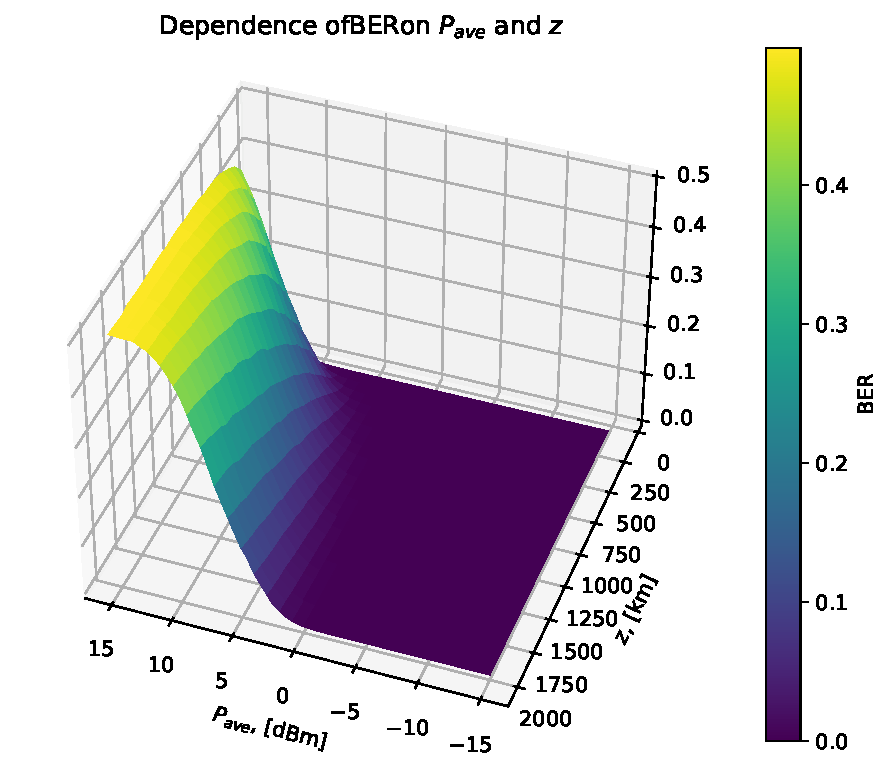
\includegraphics[width=1\linewidth]{images/benchmark/ber_vs_p_ave_dbm_3d_wo_noise.pdf} (a) 
    }
    \end{minipage}
    \hfill
    \begin{minipage}[h]{0.5\linewidth}
    \center{
        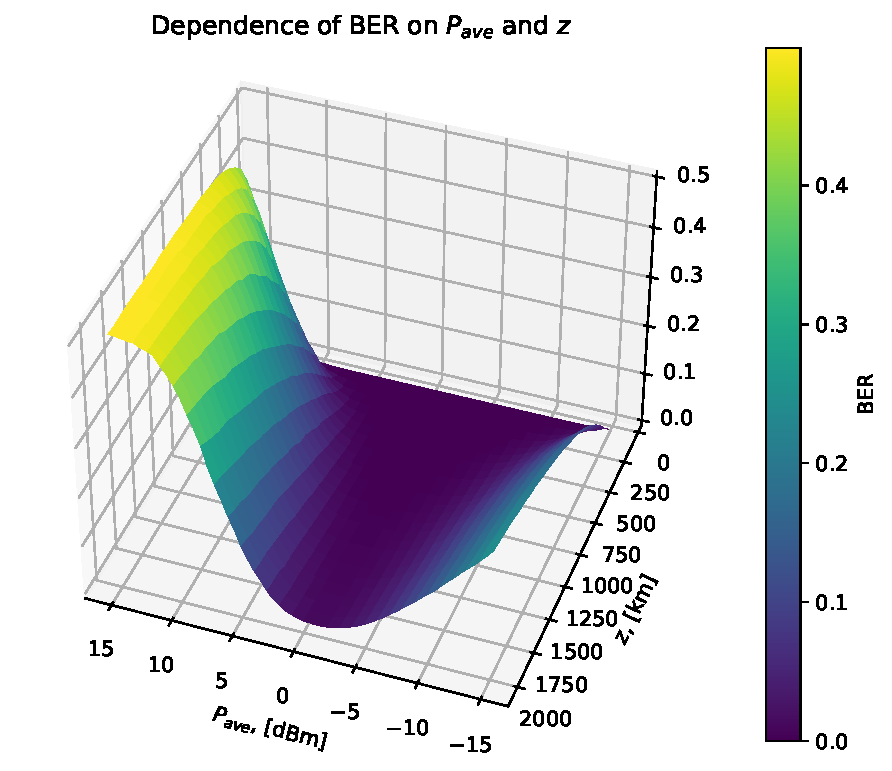
\includegraphics[width=1\linewidth]{images/benchmark/ber_vs_p_ave_dbm_3d.pdf} (b) 
    }
    \end{minipage}

    \begin{minipage}[h]{0.5\linewidth}
    \center{
        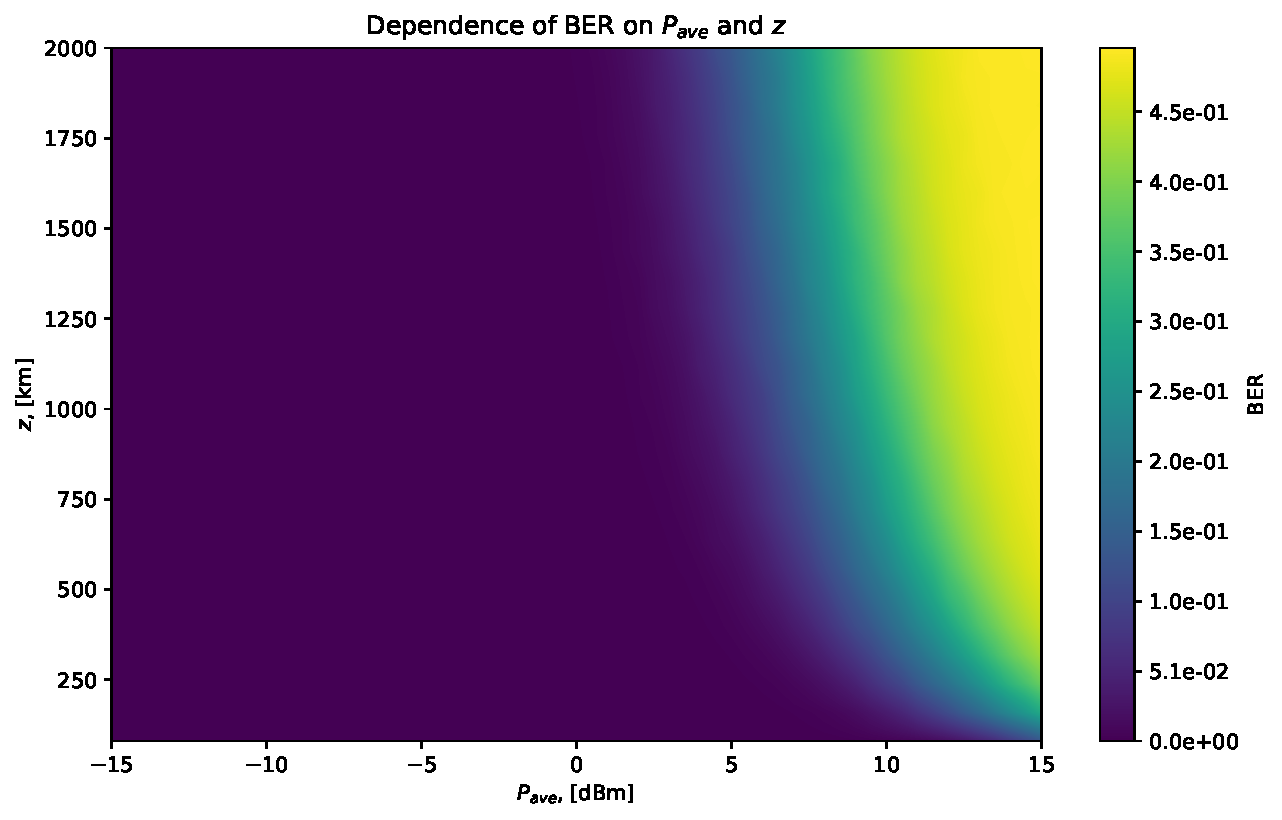
\includegraphics[width=1\linewidth]{images/benchmark/ber_vs_p_ave_dbm_2d_wo_noise.pdf} (c) 
    }
    \end{minipage}
    \hfill
    \begin{minipage}[h]{0.5\linewidth}
    \center{
        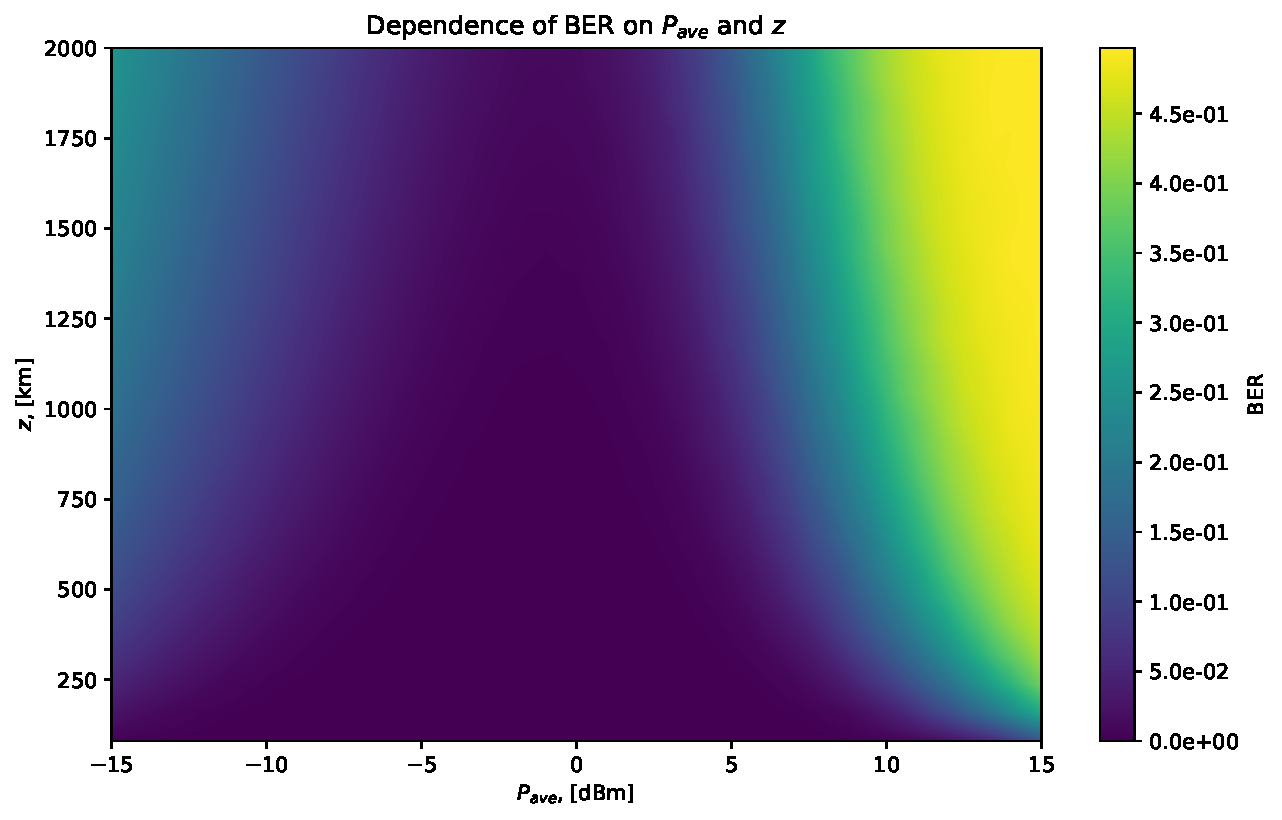
\includegraphics[width=1\linewidth]{images/benchmark/ber_vs_p_ave_dbm_2d.pdf} (d) 
    }
    \end{minipage}

    \begin{minipage}[h]{0.5\linewidth}
    \center{
        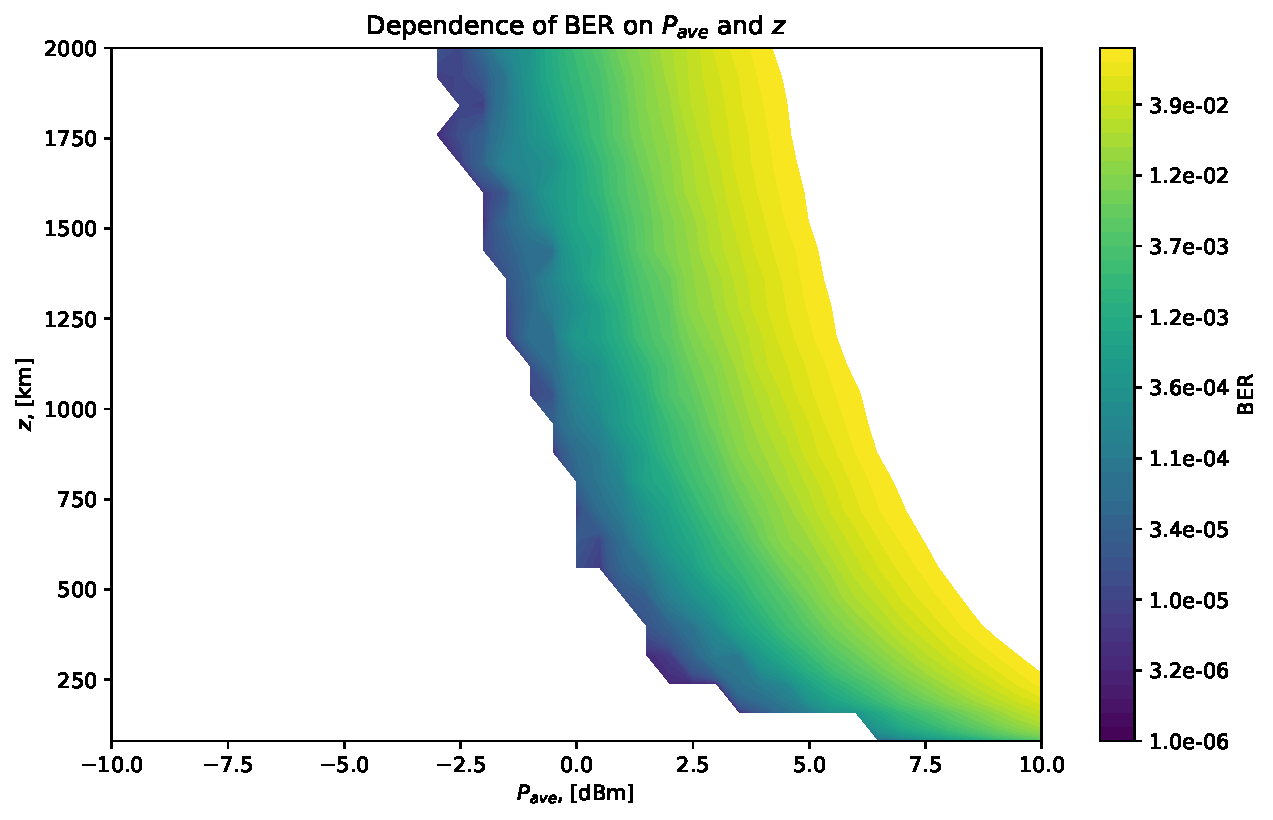
\includegraphics[width=1\linewidth]{images/benchmark/ber_vs_p_ave_dbm_2d_cut_wo_noise.pdf} (e) 
    }
    \end{minipage}
    \hfill
    \begin{minipage}[h]{0.5\linewidth}
    \center{
        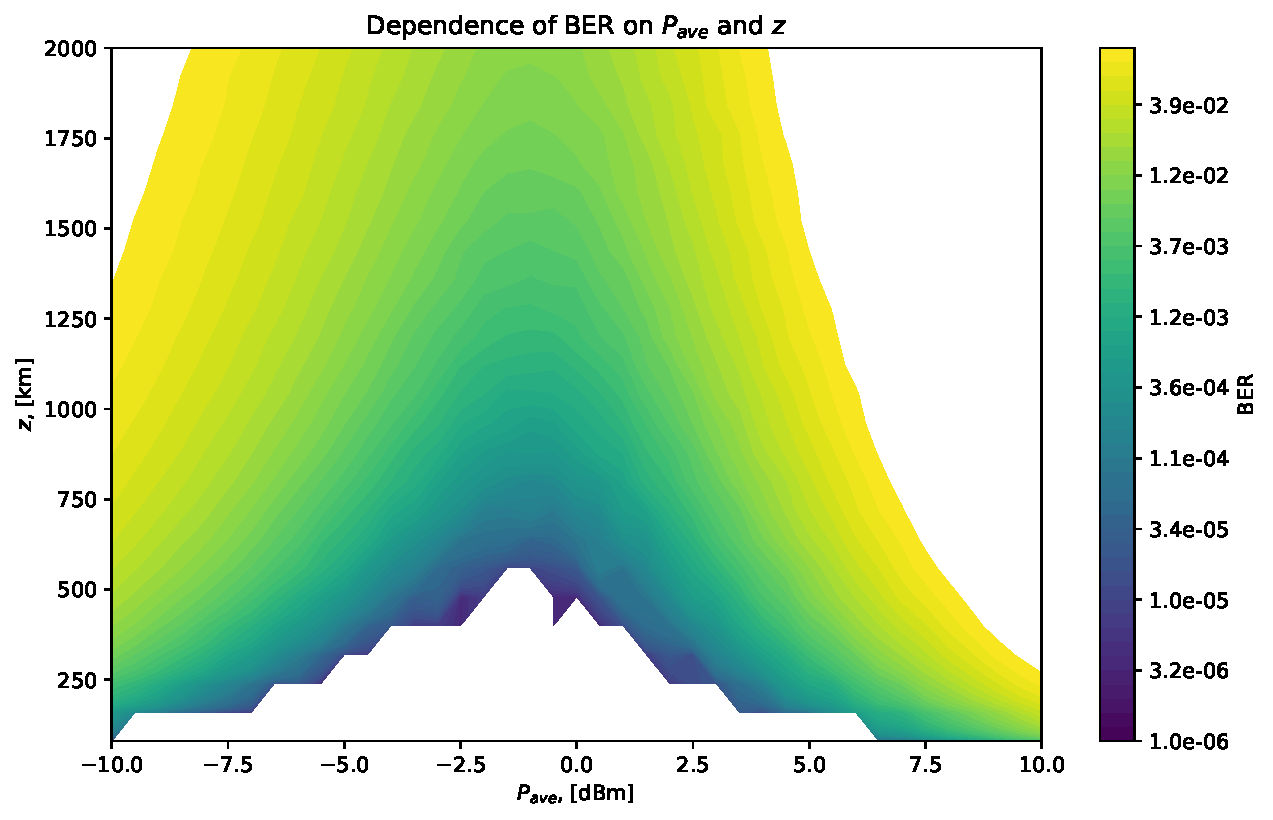
\includegraphics[width=1\linewidth]{images/benchmark/ber_vs_p_ave_dbm_2d_cut.pdf} (f)
    }
    \end{minipage}
    \caption{16-QAM. Lenght of the fiber changes from 80 km to 2000 km (from 1 span of fibre up to 25 spans). Signal average power changes from -15 dBm up to 15 dBm (with step of 0.5 dBm). Left column represents the case where there is no additional EDFA noise, right column - 4.5 dB EDFA noise figure. For each set of parameters there is $2^{16}$ symbols.}
    \label{fig:hpcom_example1}
\end{figure}


% We can see the difference between Fig.~\ref{fig:hpcom_example1} and Fig.~\ref{fig:hpcom_example2}. For higher modulation format (256-\acrshort{qam}, Fig.~\ref{fig:hpcom_example2}) the regeon with low \gls{ber} are much narrow. Moreover third row shows that in this case we doesnot reach lower \acrshort{ber} level of $10^{-6}$. 

The contrast between Fig.~\ref{fig:hpcom_example1} and Fig.~\ref{fig:hpcom_example2} is noticeable. In the case of the higher modulation format, 256-\acrshort{qam} shown in Fig.~\ref{fig:hpcom_example2}, the range where we have a low \gls{ber} is much narrower. Additionally, the third row indicates that, for this higher modulation format, we do not achieve a \acrshort{ber} as low as $10^{-6}$.



\begin{figure}[htpb]
    \begin{minipage}[h]{0.48\linewidth}
    \center{
        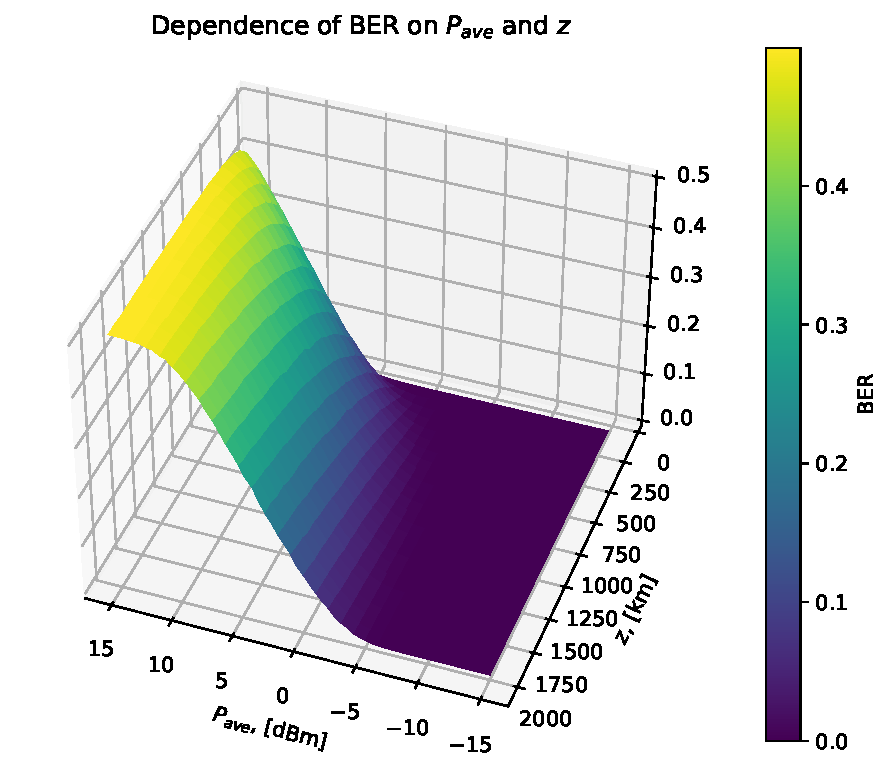
\includegraphics[width=1\linewidth]{images/benchmark/ber_vs_p_ave_dbm_3d_wo_noise_1ch_256qam.pdf} (a) 
    }
    \end{minipage}
    \hfill
    \begin{minipage}[h]{0.48\linewidth}
    \center{
        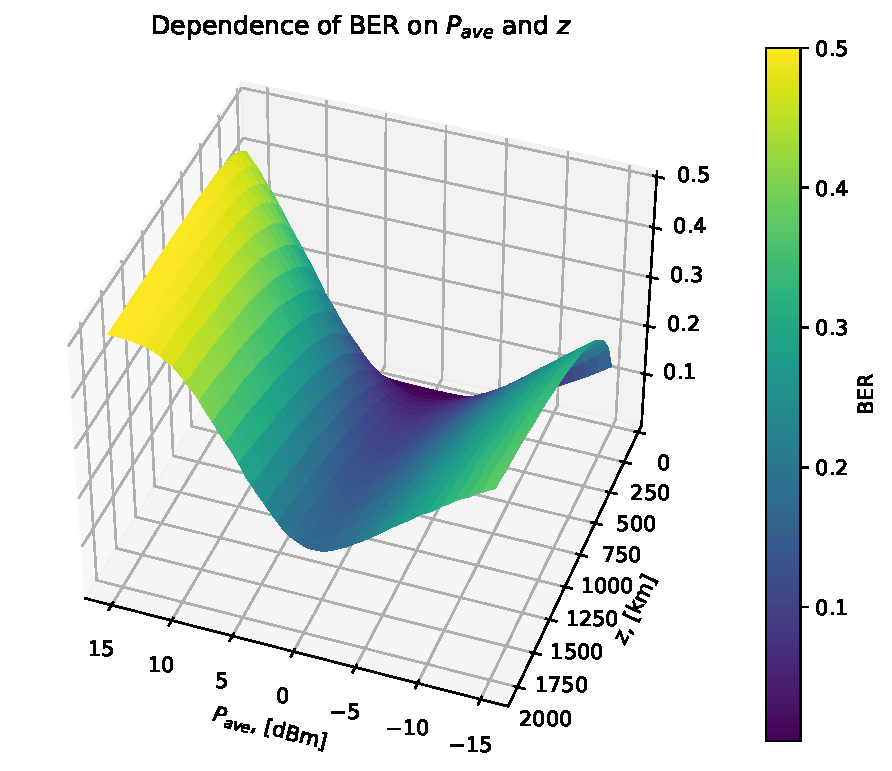
\includegraphics[width=1\linewidth]{images/benchmark/ber_vs_p_ave_dbm_3d_1ch_256qam.pdf} (b) 
    }
    \end{minipage}

    \begin{minipage}[h]{0.48\linewidth}
    \center{
        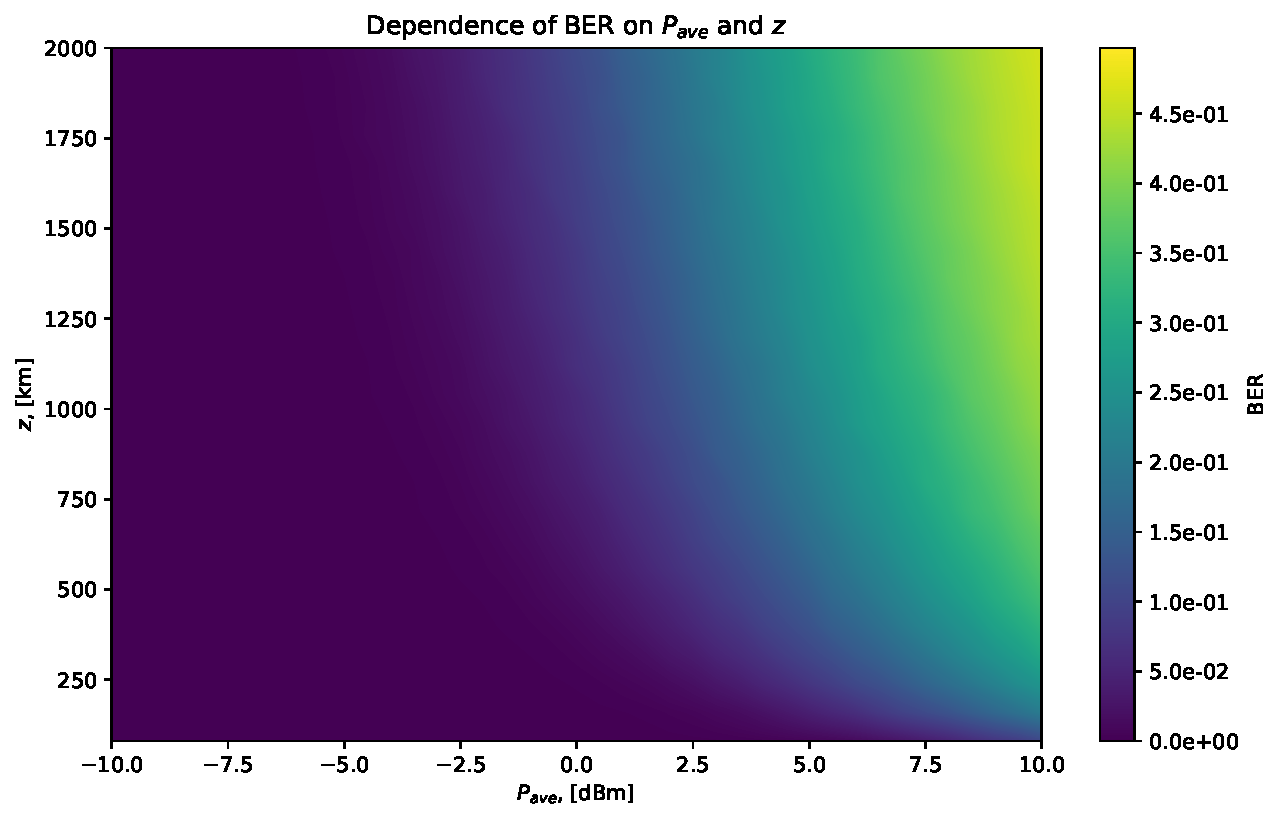
\includegraphics[width=1\linewidth]{images/benchmark/ber_vs_p_ave_dbm_2d_wo_noise_1ch_256qam.pdf} (c) 
    }
    \end{minipage}
    \hfill
    \begin{minipage}[h]{0.48\linewidth}
    \center{
        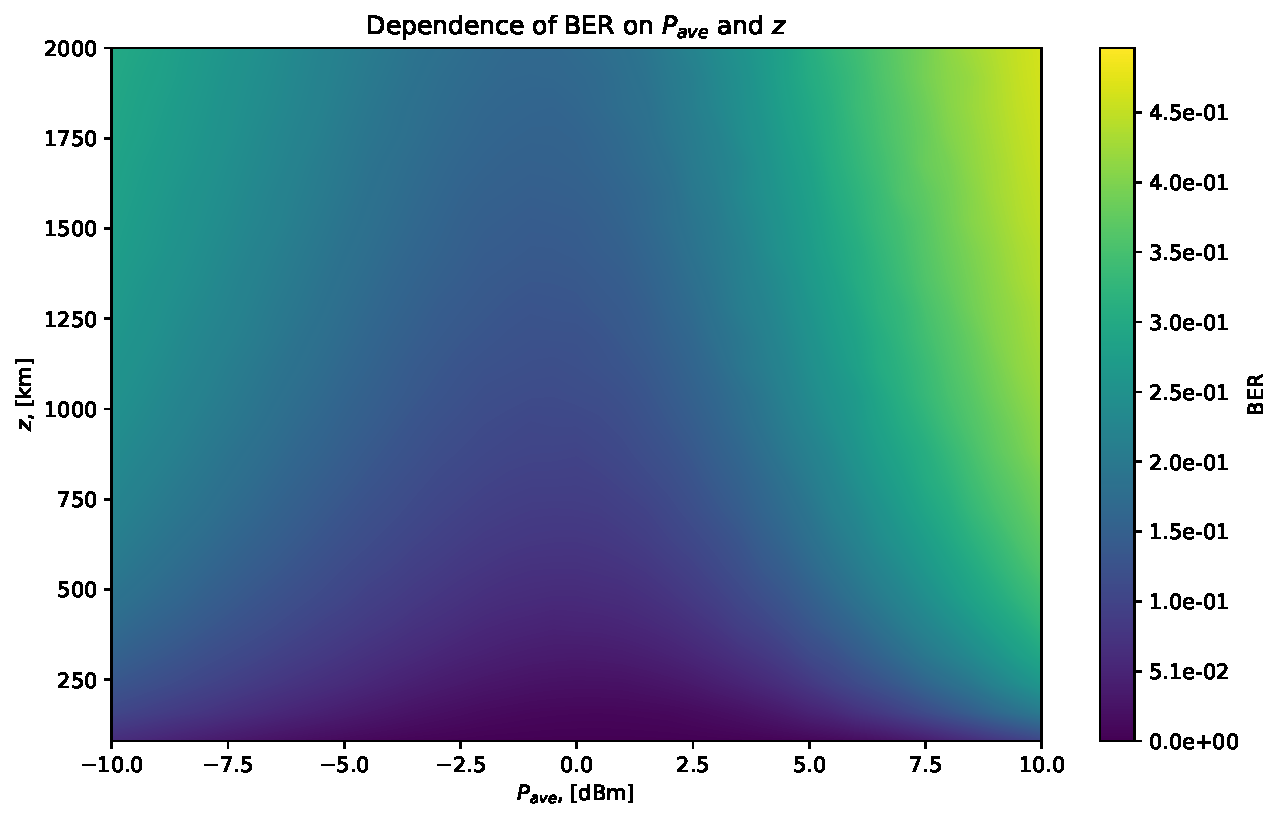
\includegraphics[width=1\linewidth]{images/benchmark/ber_vs_p_ave_dbm_2d_1ch_256qam.pdf} (d) 
    }
    \end{minipage}

    \begin{minipage}[h]{0.48\linewidth}
    \center{
        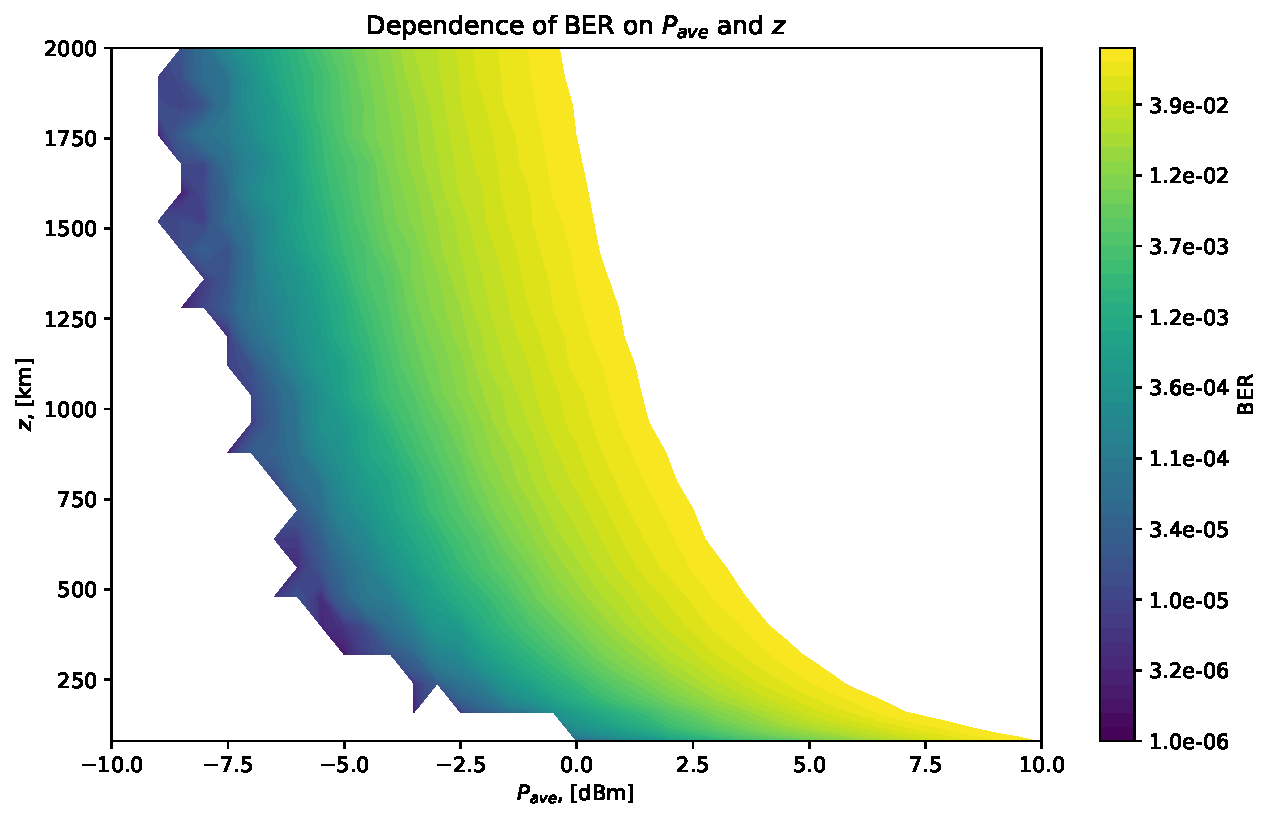
\includegraphics[width=1\linewidth]{images/benchmark/ber_vs_p_ave_dbm_2d_cut_wo_noise_1ch_256qam.pdf} (e)
    }
    \end{minipage}
    \hfill
    \begin{minipage}[h]{0.48\linewidth}
    \center{
        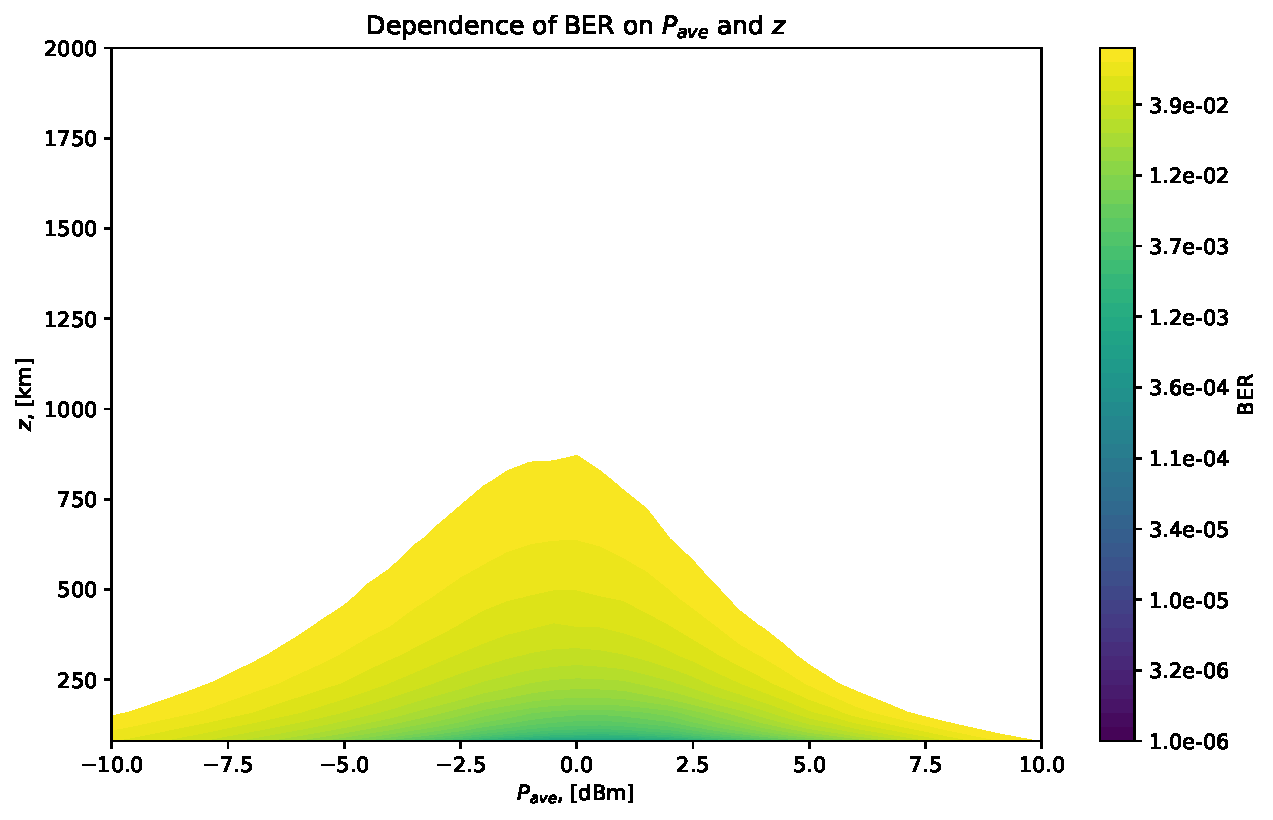
\includegraphics[width=1\linewidth]{images/benchmark/ber_vs_p_ave_dbm_2d_cut_1ch_256qam.pdf} (f)
    }
    \end{minipage}
    \caption{256-QAM. Lenght of the fiber changes from 80 km to 2000 km (from 1 span of fibre up to 25 spans). Signal average power changes from -15 dBm up to 15 dBm (with step of 0.5 dBm). Left column represents the case where there is no additional EDFA noise, right column - 4.5 dB EDFA noise figure. For each set of parameters there is $2^{16}$ symbols.}
    \label{fig:hpcom_example2}
\end{figure}



\section{Conclusion}
The GPU-accelerated framework presents a marked improvement in performance over CPU-based implementations, especially for larger problem sizes and complex simulations. The significant speedup achieved with GPU acceleration underscores its wide-ranging benefits in various aspects of optical communication system simulations, such as advanced research, high-dimensional optimization problems, swift validation of theoretical concepts, and adjustment of simulation parameters. Moreover, the accelerated framework facilitates efficient data mining, laying the groundwork for machine learning applications and the development of intelligent systems within the field. This user-friendly, versatile, and powerful framework empowers researchers to concentrate on innovation, ultimately boosting productivity and paving the way for groundbreaking discoveries in the realm of optical communication.